\documentclass[../../main.tex]{subfiles}

% Image numbers: 10-201 inclusive
% NOTE: present tense

\begin{document}

\newchapter{Final Design Proposal}{final-design-proposal}

\section{Wing} \label{sec:final-design-proposal:wing}

The wing assembly was designed to be unfastened from the fuselage assembly with ease.
Such a decision was established so as to reduce the encumbrance of the UAV during transportation.
The wing assembly is comprised of two carbon spars placed respectively at quarter and half chord, and extending for the entire \metres{2} wingspan, each half of the wing containing three ribs (Figure \ref{fig:ribs}).
These ribs fulfil multiple functions in the wing assembly and will be discussed in further detail later.
The use of profiles carved out of blue styrofoam (extruded polystyrene) provide a lightweight structure for the aerodynamic profiles such as flaps, aileron, and wing itself.
A hollow profile also allows the fitting of wires in the wing structure.
A central mounting plate provides the fitting points for the fastening of the wing assembly to the fuselage.

\subsection{Spars} \label{sec:final-design-proposal:wing:spars}

The two-spar structure utilised for the wind tunnel model's wing exhibited only small deflections in bending and twist when tested, and this same configuration is therefore maintained for the flight model.
Two carbon spars are used for the final design, thus reducing the weight while maintaining the same structural characteristics.
These were sized for a loading case equal to $4g$, at which the wing would present a deflection of \mm{54} at the wing tip as can be seen in Figure \ref{fig:fea-half-wingspan}.
Both spars have a wall thickness of \mm{2} whereas their diameters differ: the first one, positioned at quarter chord, has a diameter of \mm{16}; while the one positioned at half chord has a diameter of \mm{14}.

\importimage{fea-half-wingspan}{FEA of half wingspan subject to a distributed load of 138N/m.}{FEA of half wingspan}{0.9}

\subsection{Ribs} \label{sec:final-design-proposal:wing:ribs}

The attachment points for the power units take the form of 3D printed inserts embedded in the wing structure.
These, as shown in Figure \ref{fig:ribs}, present the same aerofoil section as the wing so as not to disrupt the airflow.
Three inserts per half wingspan allow as many different propulsion positions as possible: \pc{20} wingspan, \pc{40} wingspan, and \pc{100} wingspan (wingtip); thus allowing the assessment of the effects of the propulsion unit placed close to the fuselage structure (\pc{20} wingspan); at the optimal position found by Kroo (\cite{kroo-86}), \pc{40} wingspan; and at the wingtip (\pc{100} wingspan).

The design of this last is mounting point is, however, different from the semi-span inserts.
For each of the semi-span inserts, the same motor unit can be mounted in four different configurations: underwing pusher, underwing tractor, overwing pusher, and overwing tractor (Figures \ref{fig:wing-mounting:underwing-pusher} through \ref{fig:wing-mounting:overwing-tractor} respectively); while for the wingtip-mounted element the number of available configurations is two: pusher and tractor (Figures \ref{fig:wing-mounting:wingtip-pusher} and \ref{fig:wing-mounting:wingtip-tractor}).
Adaptors are adopted to blend the standardised connection surface of the motor housing with the wing's surface, thus reducing the aerodynamic footprint. 

% \importimage{mid-span-rib}{mid-span rib.}{Mid-span rib}{0.5}
% \importimage{tip-rib}{tip rib.}{Tip rib}{0.5}

\begin{figure}[H]
    \centering
    \begin{subfigure}[b]{0.49\columnwidth}
        \centering
        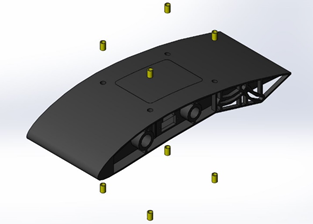
\includegraphics[width=\textwidth]{mid-span-rib}
        \caption{Mid-span}
        \label{fig:ribs:mid-span}
    \end{subfigure}
    \hfill
    \begin{subfigure}[b]{0.49\columnwidth}
        \centering
        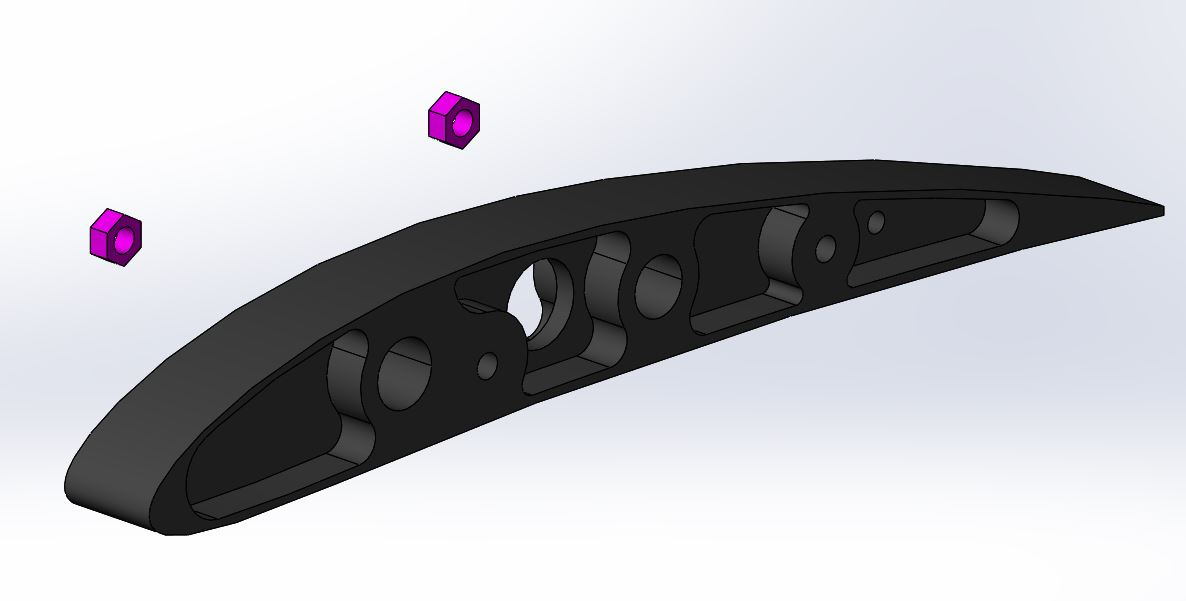
\includegraphics[width=\textwidth]{tip-rib}
        \caption{Tip}
        \label{fig:ribs:tip}
    \end{subfigure}
    
    \caption{CAD models of the wing ribs.}
    \label{fig:ribs}
\end{figure}

% \importimage{underwing-pusher}{underwing pusher configuration.}{Underwing pusher}{0.5}
% \importimage{underwing-tractor}{underwing tractor configuration.}{Underwing tractor}{0.5}
% \importimage{overwing-pusher}{overwing pusher configuration.}{Overwing pusher}{0.5}
% \importimage{overwing-tractor}{overwing tractor configuration.}{Overwing tractor}{0.5}
% \importimage{wingtip-pusher}{wingtip pusher configuration.}{Wingtip pusher}{0.5}
% \importimage{wingtip-tractor}{wingtip tractor configuration.}{Wingtip tractor}{0.5}

\begin{figure}[H]
    
    \centering
    \begin{subfigure}[b]{0.49\columnwidth}
        \centering
        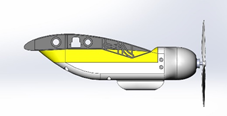
\includegraphics[width=\textwidth]{underwing-pusher}
        \caption{Underwing pusher}
        \label{fig:wing-mounting:underwing-pusher}
    \end{subfigure}
    \hfill
    \begin{subfigure}[b]{0.49\columnwidth}
        \centering
        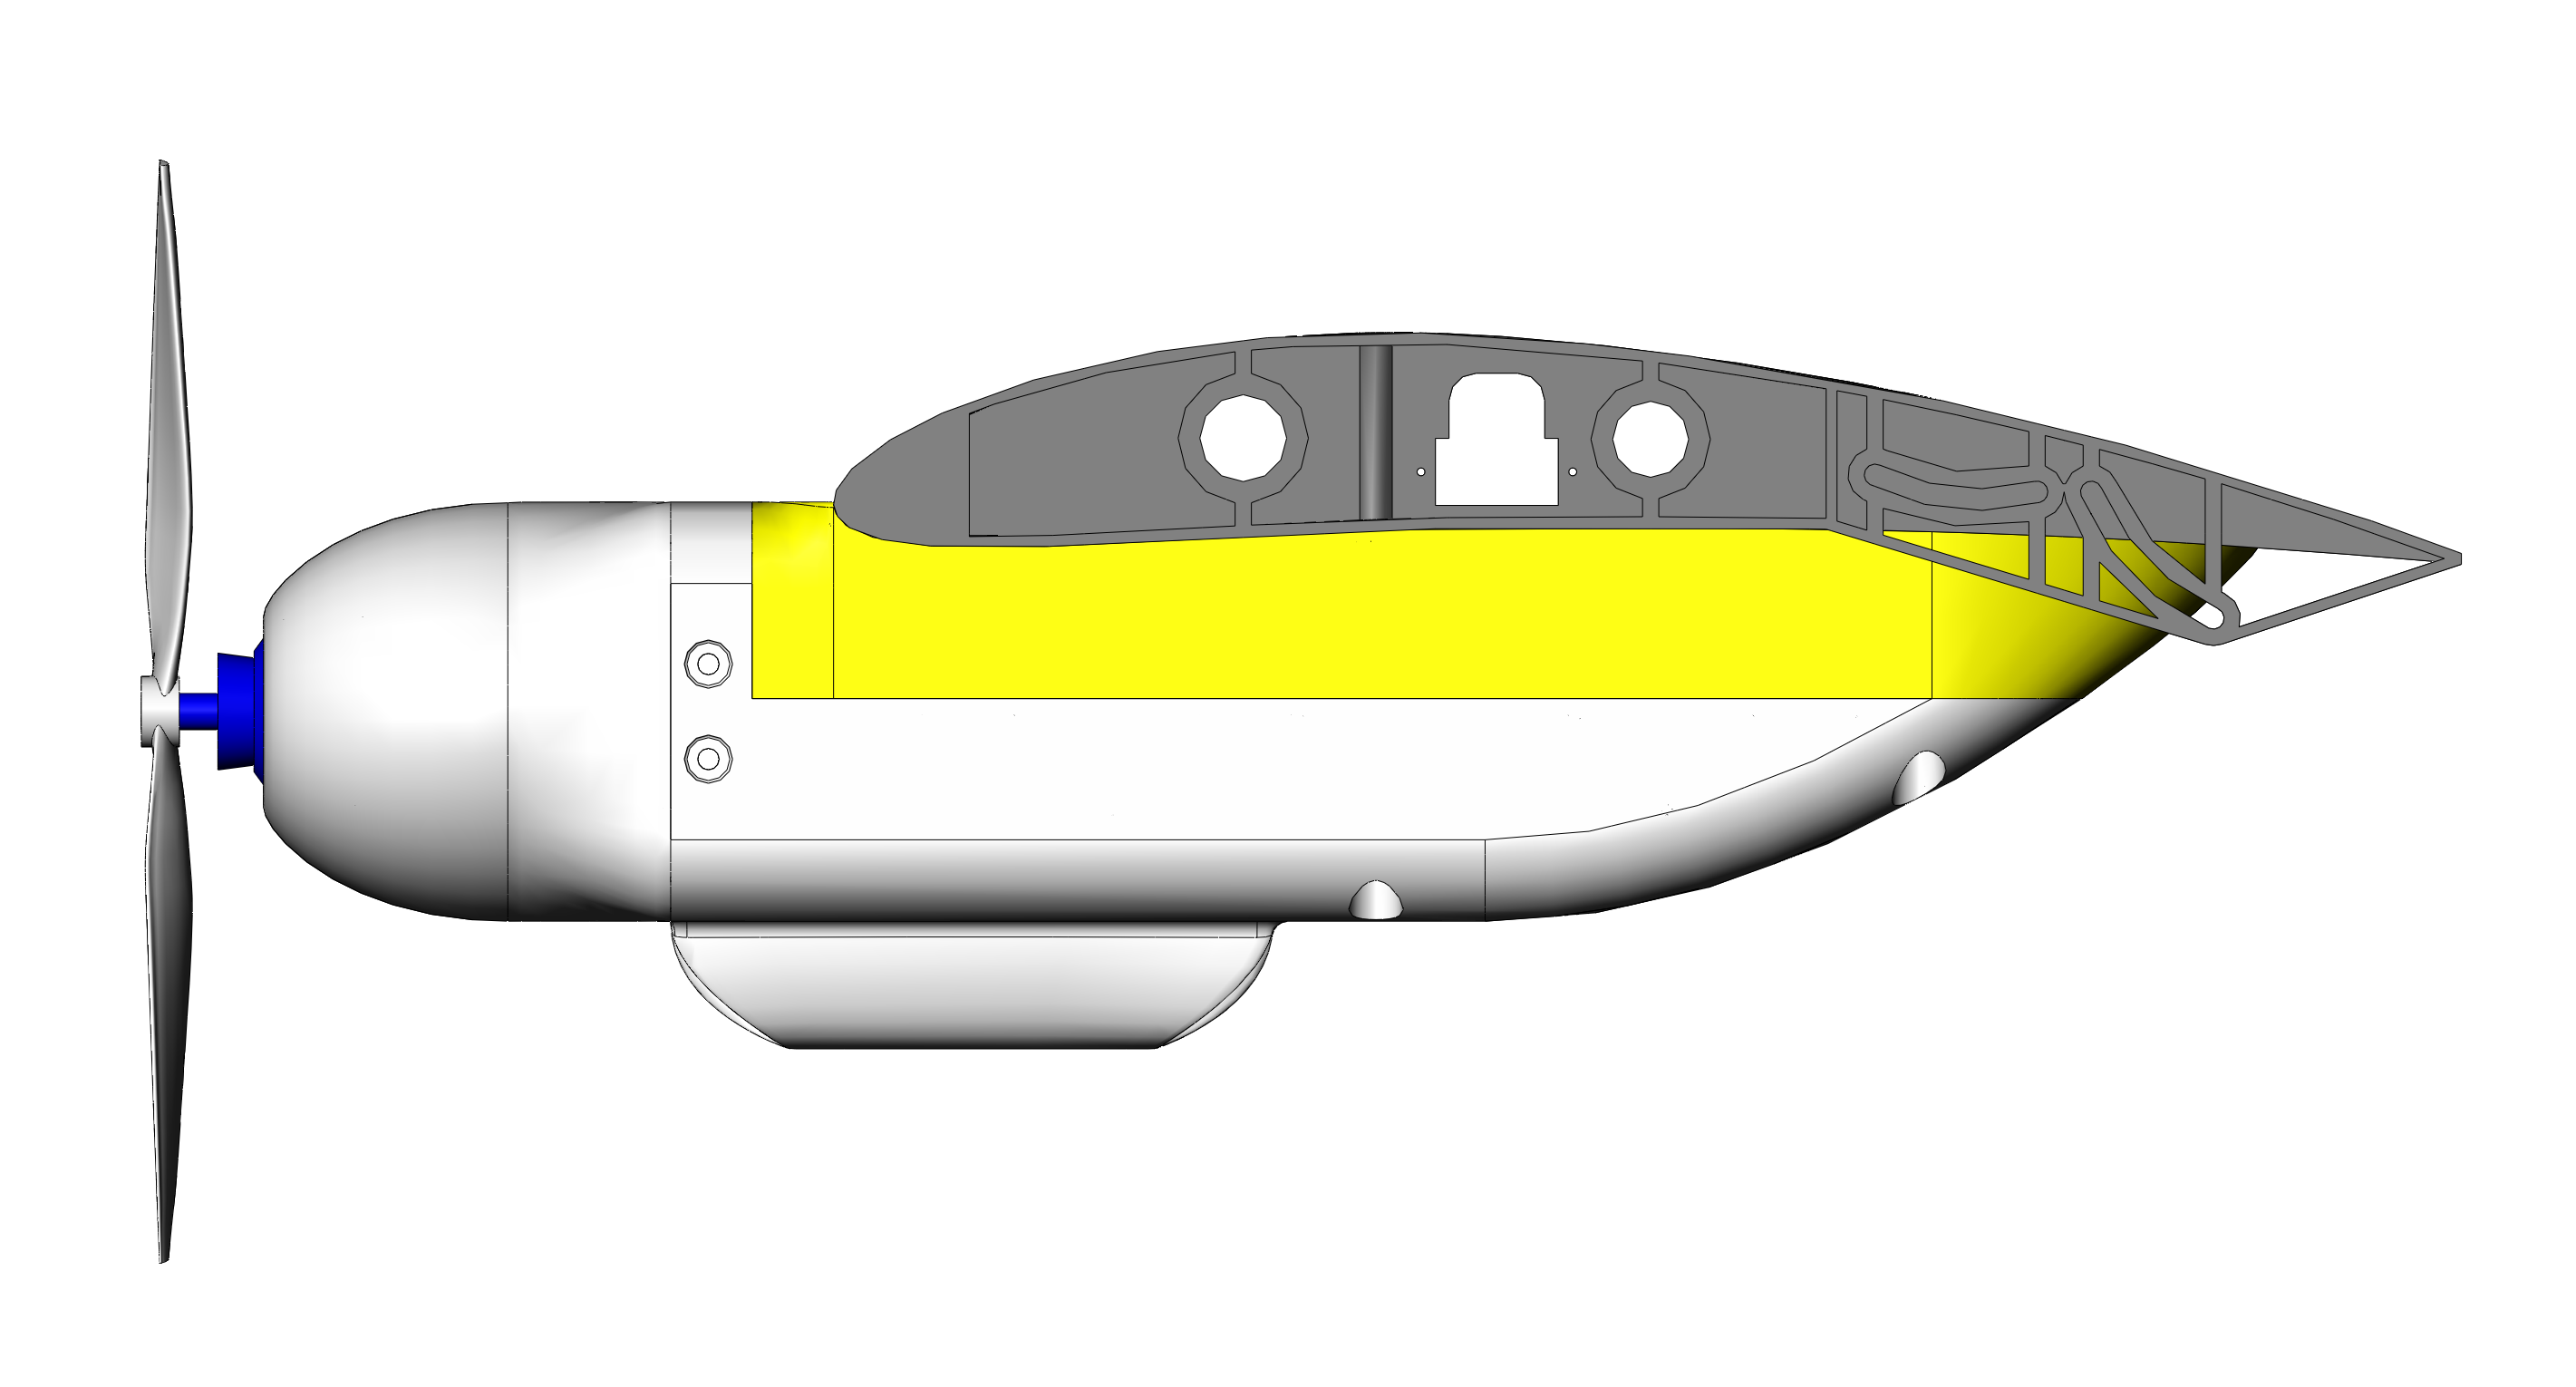
\includegraphics[width=\textwidth]{underwing-tractor}
        \caption{Underwing tractor}
        \label{fig:wing-mounting:underwing-tractor}
    \end{subfigure}
    
    \centering
    \begin{subfigure}[b]{0.49\columnwidth}
        \centering
        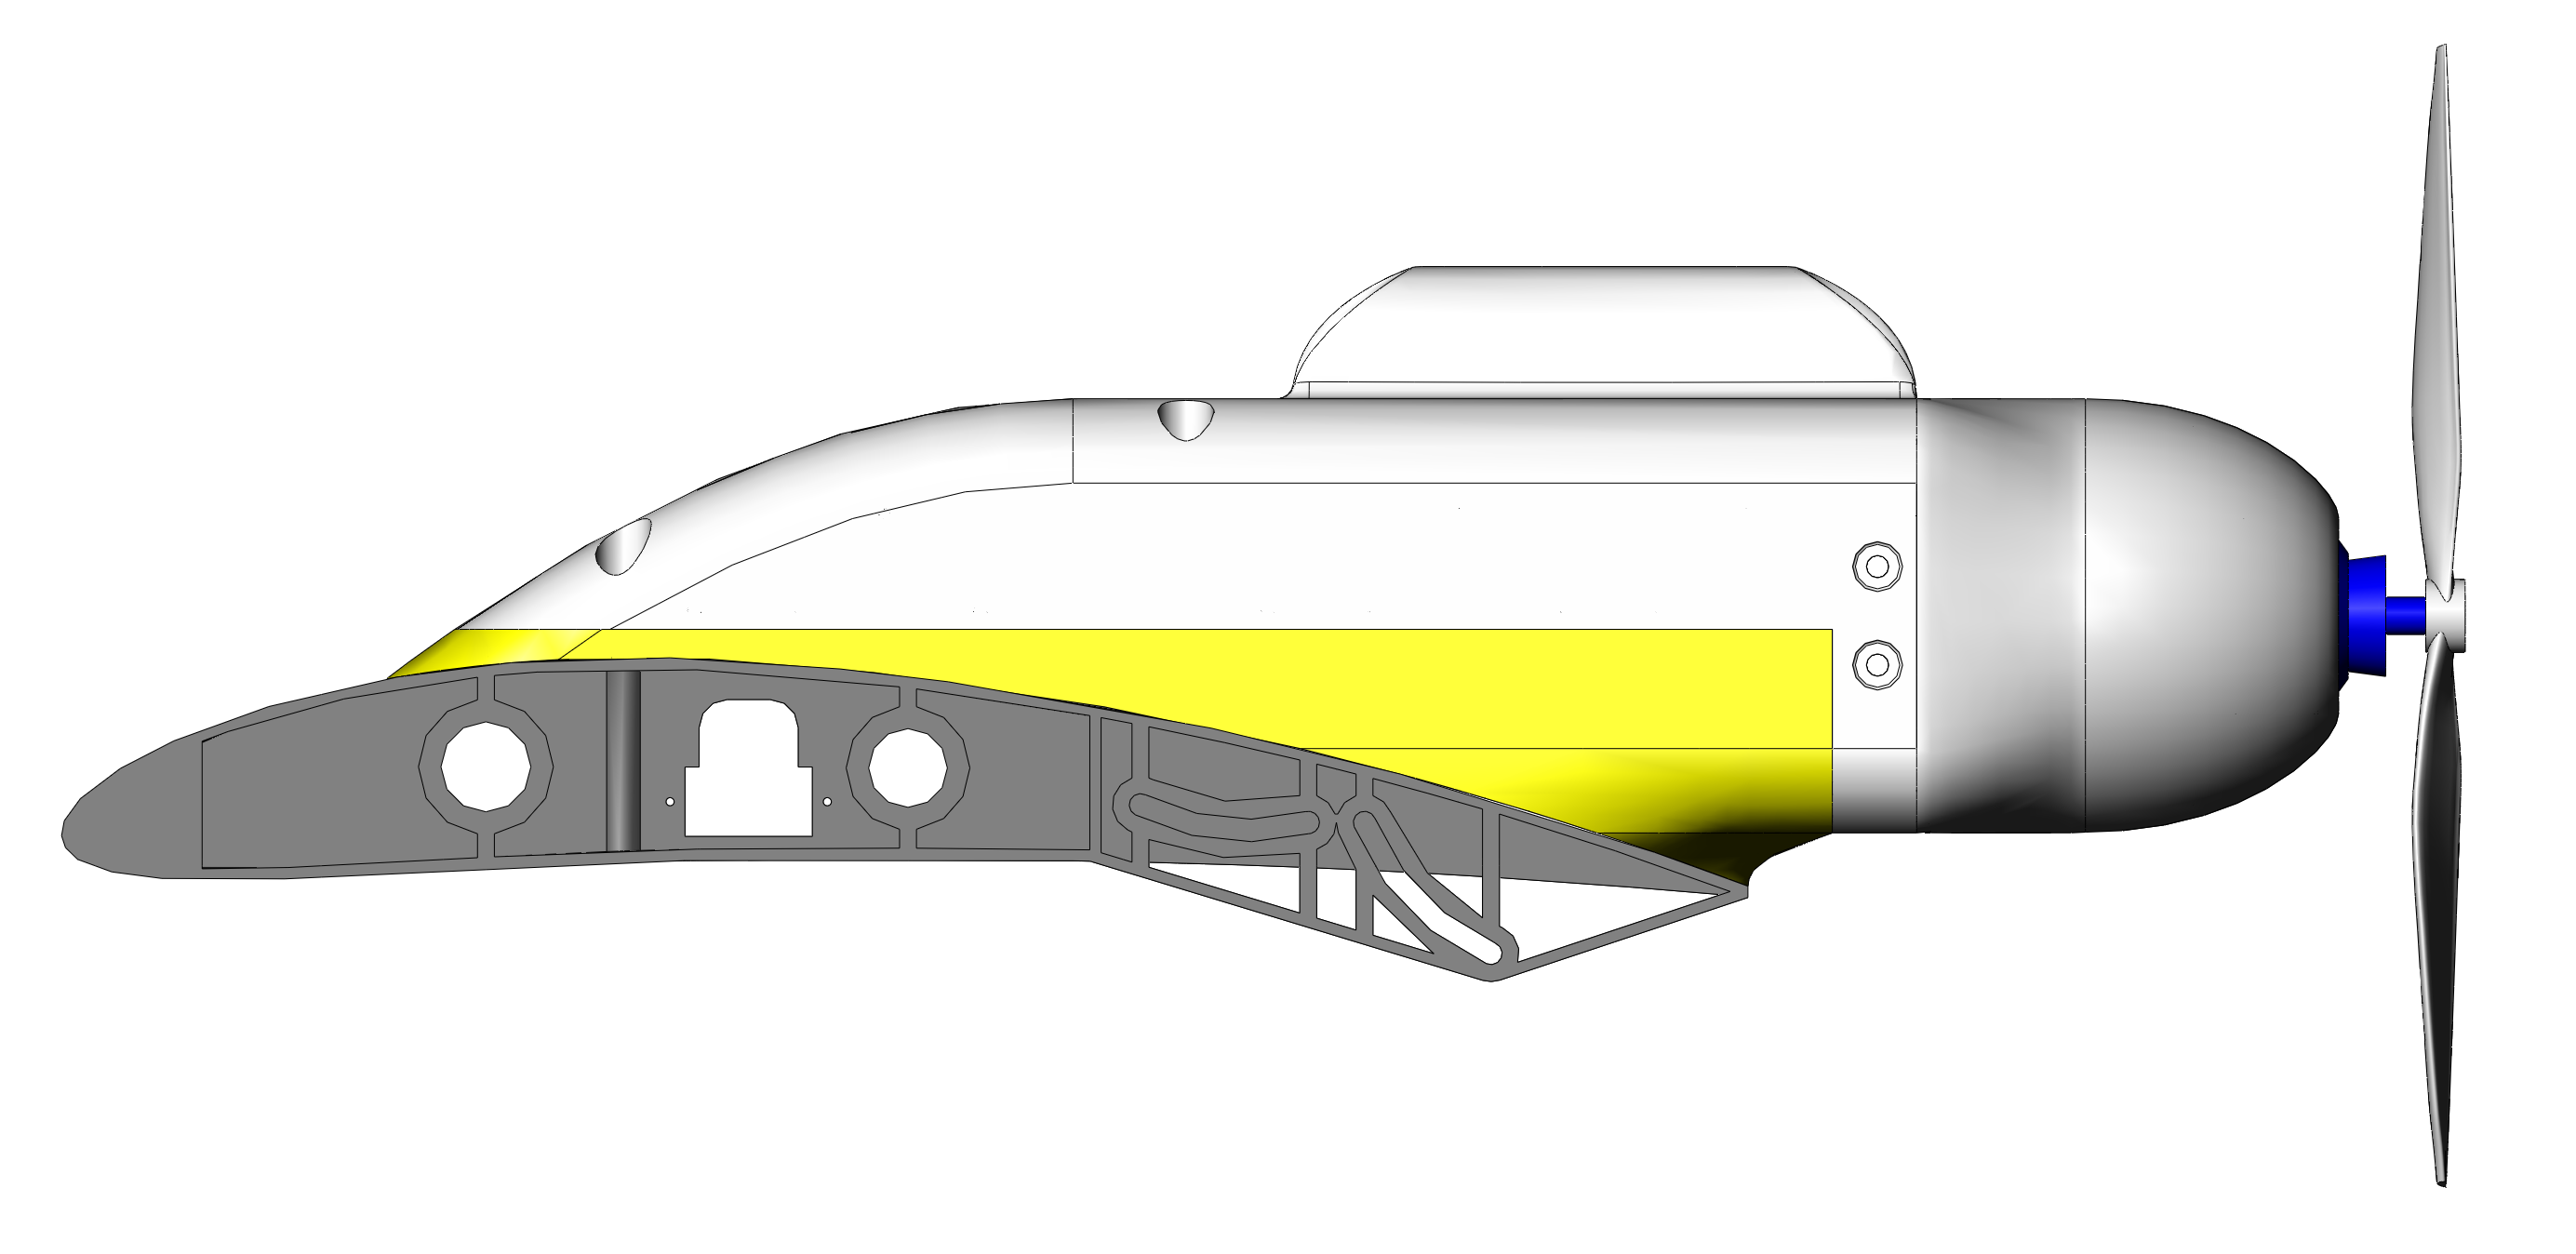
\includegraphics[width=\textwidth]{overwing-pusher}
        \caption{Overwing pusher}
        \label{fig:wing-mounting:overwing-pusher}
    \end{subfigure}
    \hfill
    \begin{subfigure}[b]{0.49\columnwidth}
        \centering
        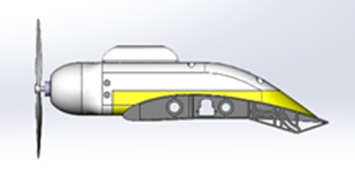
\includegraphics[width=\textwidth]{overwing-tractor}
        \caption{Overwing tractor}
        \label{fig:wing-mounting:overwing-tractor}
    \end{subfigure}
    
    \centering
    \begin{subfigure}[b]{0.49\columnwidth}
        \centering
        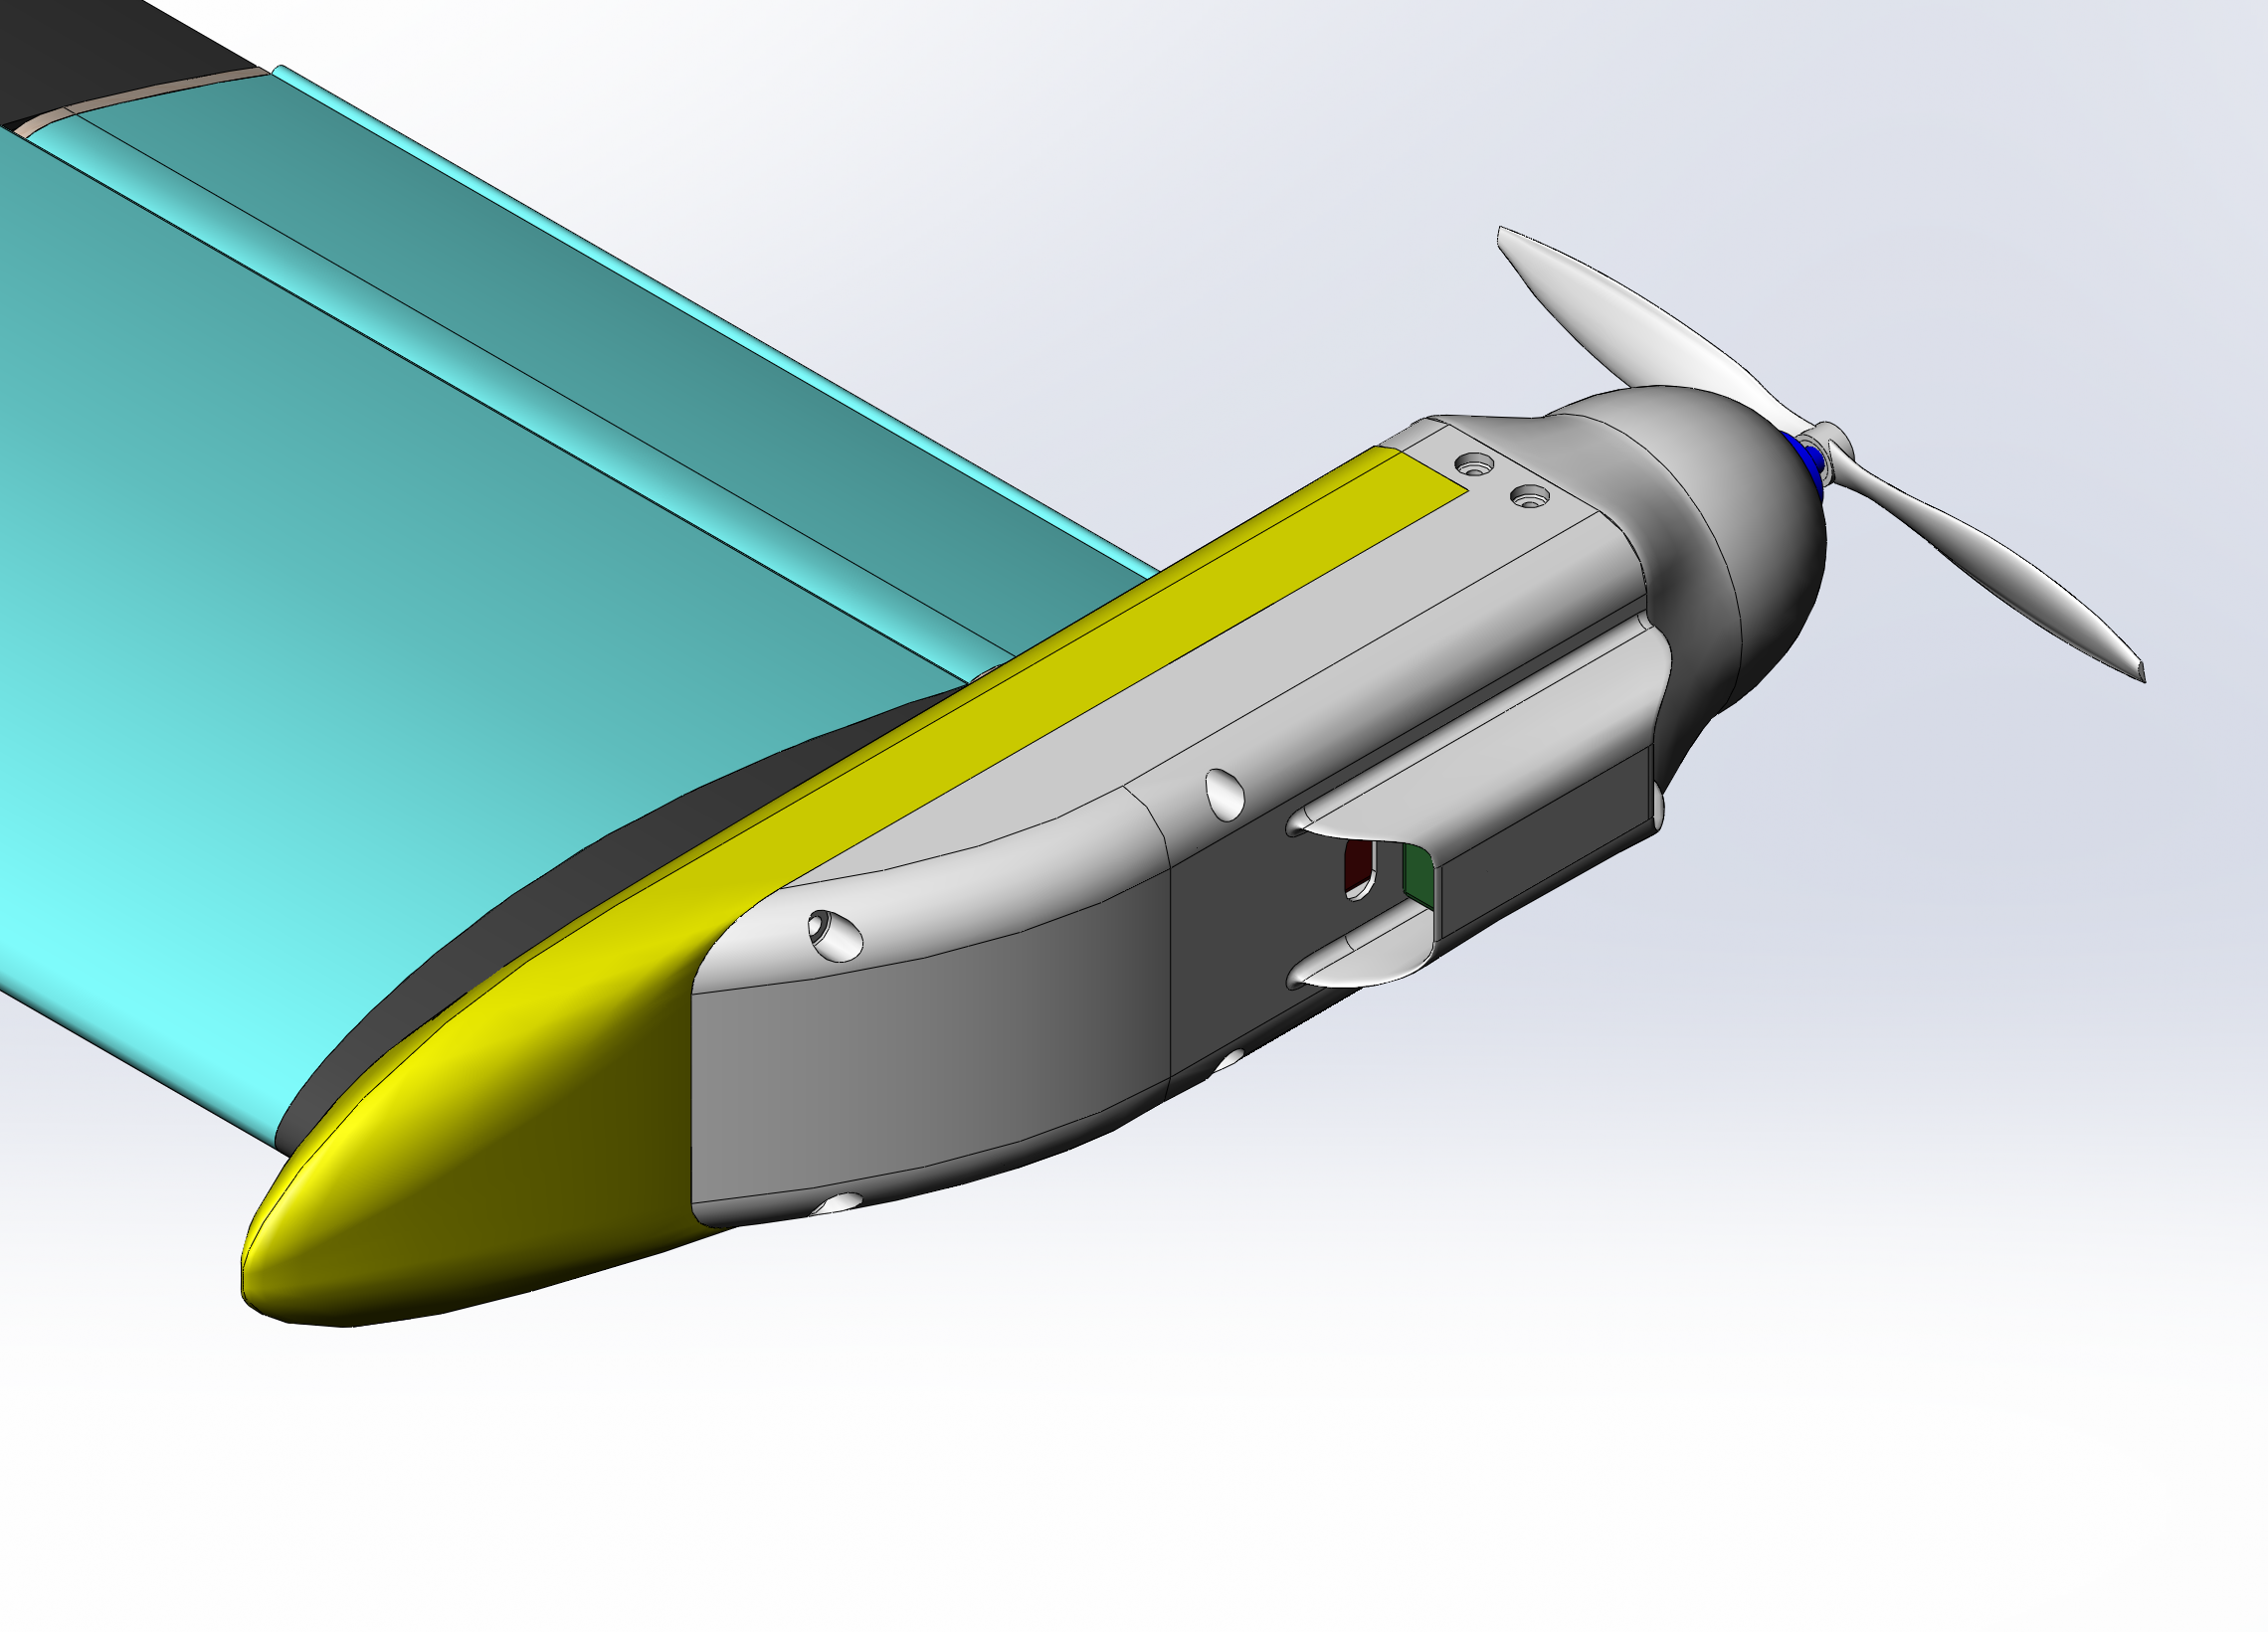
\includegraphics[width=\textwidth]{wingtip-pusher}
        \caption{Wingtip pusher}
        \label{fig:wing-mounting:wingtip-pusher}
    \end{subfigure}
    \hfill
    \begin{subfigure}[b]{0.49\columnwidth}
        \centering
        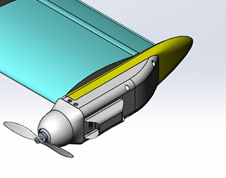
\includegraphics[width=\textwidth]{wingtip-tractor}
        \caption{Wingtip tractor}
        \label{fig:wing-mounting:wingtip-tractor}
    \end{subfigure}
    
    \caption{possible configurations of the PUC on the wing mounts.}
    \label{fig:wing-mounting}
\end{figure}

Each semi-span insert is equipped with four brass threaded inserts on both the top and bottom surfaces.
These permit the fastening of the power unit cells and the respective adapter.
The location of the holes is the same for top and bottom surface (when viewed from the top).
As such, the same motor housing can be mounted on the top and bottom surface without alterations.
Furthermore, as presented in Figure \ref{fig:wing-insert}, the inserts are equidistant from the centreline positioned at half chord, thereby allowing the mounting of the same power unit cell (PUC) in tractor or pusher configurations without the need for alterations. 

\importimage{wing-insert}{section view of the wing insert.}{Wing insert}{0.9}

The tip insert is designed to mount the motor housing in a horizontal orientation.
In order to use the same configuration of mounting points the tip adaptor covers a structural role, unlike the others.
This presents the brass inserts configuration discussed above so to guarantee the attachment of the standardized PUC.  % TODO: clarify meaning
The adapter is then mounted to the insert though two M6 bolts fastened to the two imbedded nuts shown in Figure \ref{fig:ribs:tip}. 

In order to reduce the number of elements comprising the wing assembly, these components cover the function of ribs as well providing further torsional rigidity to the wing structure.
The two holes shown in Figure \ref{fig:wing-insert} permit the carbon spars to run through the rib insert, providing a secure attachment and sufficient bonding area.
Furthermore, as will be discussed in more detail later, the housing for the active surfaces' servos and flap guides are designed to be an integral part of the rib structure. 

\subsection{Mounting plate} \label{sec:final-design-proposal:wing:mounting-plate}

A nylon printed mounting plate is located at the centre of the wing assembly and is tightly mounted to the wing spars so as to guarantee a rigid support.
The wing assembly is then clamped onto the fuselage attachment plate by four M6 bolts.
These are positioned at the corners of the 3D printed plate as shown in Figure \ref{fig:wing-assembly}.
A styrofoam cover placed on top of the mounting plate is responsible for the blending of the wing assembly with the rest of the fuselage. 

\importimage{wing-assembly}{exploded view of the wing assembly attachment procedure}{Wing assembly attachment}{0.8}

The two cylinders housing the carbon spars (Figure \ref{fig:wing-plate:cad}) ensure an even distribution of the loads though a large area.
This is essential since this component is subject to the entirety of the load transferring from the wing to the fuselage and vice versa.
Extensive work was therefore conducted using finite element analysis to generate a reliable and light design.
The peak loading for this component was established to be $4g$, simulating an abrupt increase in lift as in Figure \ref{fig:wing-plate:fea}, and producing the optimal design that was eventually used. 

% \importimage{wing-plate-cad}{CAD representation of the wing mounting plate.}{Wing mounting plate CAD}{0.6}
% \importimage{wing-plate-fea}{stress concentration due to an applied load of 275 N.}{Wing mounting plate FEA}{0.6}

\begin{figure}[H]

    \centering
    \begin{subfigure}[b]{0.49\columnwidth}
        \centering
        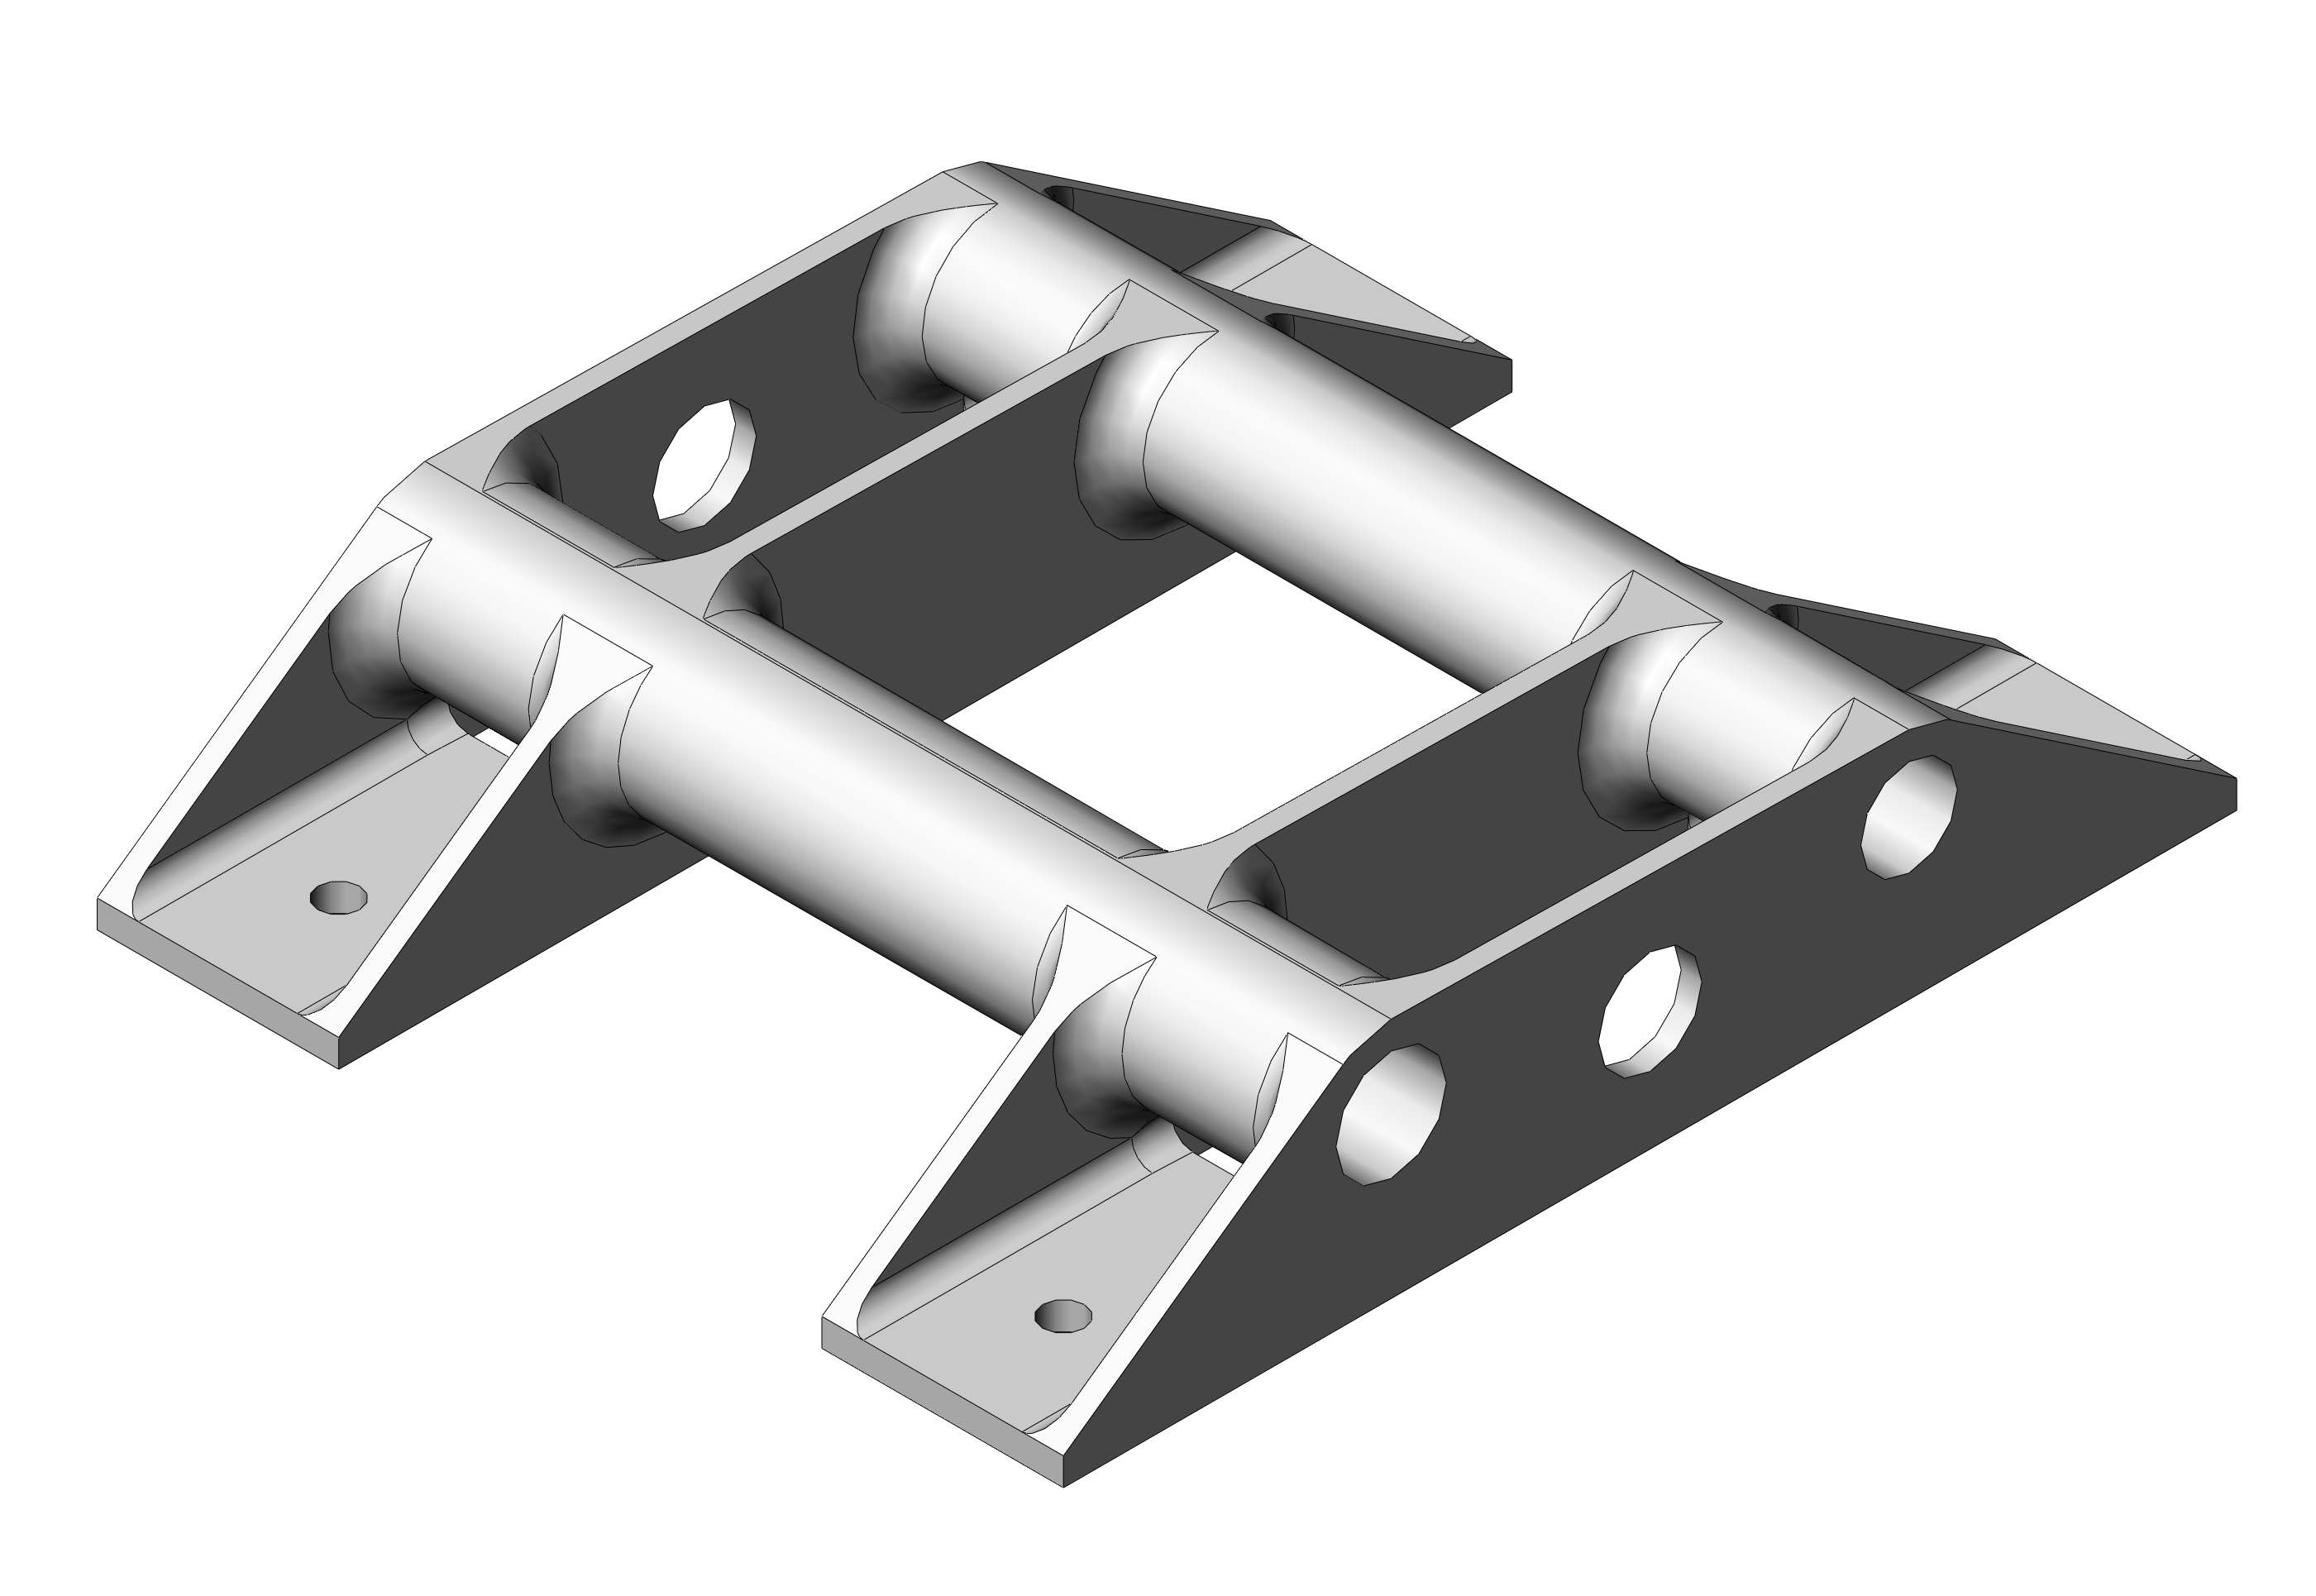
\includegraphics[width=\textwidth]{wing-plate-cad}
        \caption{CAD}
        \label{fig:wing-plate:cad}
    \end{subfigure}
    \hfill
    \begin{subfigure}[b]{0.49\columnwidth}
        \centering
        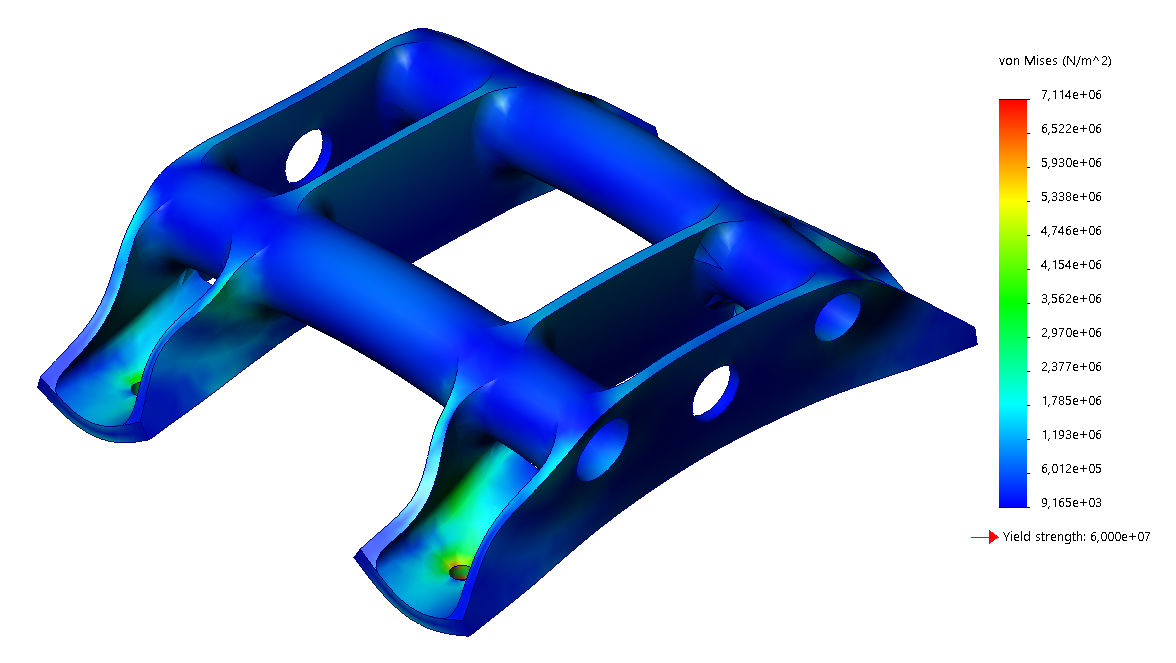
\includegraphics[width=\textwidth]{wing-plate-fea}
        \caption{FEA}
        \label{fig:wing-plate:fea}
    \end{subfigure}
    
    \caption{
        models of the wing mounting plate; (b) shows the stress concentration under a \newtons{275} load.
    }
    \label{fig:wing-plate}
\end{figure}

\subsection{Flap mathematical modelling} \label{sec:final-design-proposal:wing:flap-mathematical-modelling}

% TODO: should this go in the design process?

Flaps were an obvious addition to aid take-off and landing.
It was decided that single slotted flaps should be used to increase flap efficiency and high lift capability.
The wing was split into three main sections between the motor mounts.
Because of the restrictions bounding wingspan, the flap-to-chord ratio was the value that was altered to change high lift performance.
It was also decided that a small symmetrical deflection of the ailerons should be used in addition to the deployment of flaps, as the flaps were limited in performance.
Converting the trailing edges of the mounting locations into additional flaps was also considered, but the increase in complexity led to the decision to shelve this idea. 

Initially, the flap geometry was parametrised by defining a chord ratio of the flaps to the wing, as well as the inboard and outboard spans of each flap.
The mathematical outcome of the process gave a required angle of the fuselage either on rotation or induced by a tail gear configuration, so work on the flaps aimed to reduce this angle, especially given the clearance required by the tail propeller and the correspondingly long tail gear. 

To mathematically model the flaps, a takeoff speed was first obtained from the previously acquired data on propulsion performance.
This initial calculation suggested that for a takeoff speed of \mps{10} it would not be possible to design the flaps around with a reasonable required incidence.
After a some discussion, it was agreed that the takeoff speed should be raised to \mps{13}. 

To analyse the flap geometry, a devised from methods introduced by Sadraey \cite{sadraey-13}.
According to table 5.15 in \cite{sadraey-13}, the increase in local sectional lift coefficient for a slotted flap is 1.3 times the chord ratio of the flap to the wing, and the increase in local sectional lift coefficient for a plain flap (such as a converted aileron) is 0.7 to 0.9; 0.7 was selected from this range to be conservative. 

It is important to note that this increase in lift coefficient is for a flap deflection of \degr{60}, which is unrealistic for this application.
Additionally, because roll authority is required in all flight phases, the full aileron deflection would not be usable for high lift gain, so a small angle of \degr{5} downwards deflection was selected.
The maximum deflection of the slotted flaps was selected as \degr{40} based on data in table 5.16 from \cite{sadraey-13}.
The increase in lift coefficient for the respective flap was then multiplied by the ratio of the maximum deflection to \degr{60}.
The value for the slotted flap was further multiplied by the chord ratio as required by this method. 

A simple version of the lift equation was then defined to account for the flap and aileron deflection at takeoff: 

% TODO: mathrm on letters
\importequation{
    \begin{aligned}
    L_{TO}  & {}= q S_{NoHLDs} (C_{L_0}+C_{L_\alpha}\alpha) \\
            & \quad + qS_f ((C_{L_0}+C_{L_\alpha}\alpha) + \Delta C_{L_f}) \\
            & \quad + qS_a ((C_{L_0}+C_{L_\alpha}\alpha) + \Delta C_{L_\alpha}) \\
            & {}= qSC_{L_0} + qSC{L_\alpha}\alpha + q S_a \Delta C_{L_\alpha} + q S_f \Delta C_{L_f}
    \end{aligned}
}{takeoff-lift}

which can be rearranged for $\alpha$:

\importequation{\alpha = \frac{L_{TO} - q S C_{L_0} - q S_a \Delta C_{L_\alpha} - q S_f \Delta C_{L_f}}{q S C_{L_\alpha}}}{rearranged-takeoff-lift}

The takeoff lift was estimated as \newtons{10} greater than the maximum takeoff weight of the UAV to provide responsive climb performance.
$S_a$ and $S_f$ were determined by multiplying the total span for the flaps and ailerons by the wing chord, and $\Delta$\cla and $\Delta$\clf from the earlier calculations.
$\alpha$ turned out to require \degr{7.88} total wing incidence on takeoff, based on the final selected value of flap to wing chord ratio of 0.4, which was the maximum reasonable value before the flaps would begin impinging on electronics or wing spars.

The wing chord line had been set at an angle of \degr{2} relative to the fuselage: the required incidence of the fuselage, either provided by the landing gear or rotation, would be $7.8768^\circ – 2^\circ = 5.8768^\circ$. 

\subsection{Flap CAD} \label{sec:final-design-proposal:wing:flap-cad}

The shape of the flap was defined from a copy of the wing CAD.
Since a slotted flap had been chosen, a shroud from the wing had to extend to near the leading edge of the flaps in a deployed position such that boundary layer re-energisation on top of the flap would be optimal.
The wing shroud had been defined in CAD, so its profile was transferred onto the flap profile, smoothed out, and then cut off from the leading edge and upper surface.  

Based on feedback on an original design, the flap mechanism of a Cessna-172 was selected as inspiration for the next version \cite{towell-19}.
Images of this mechanism were studied, and a mechanism designed producing a smooth deployment both translationally back and down, and rotationally back to the \degr{40} angle specified. 

\importimage{flap-mechanism-side}{the flap mechanism.}{Flap mechanism side view}{0.6}

The pins were made as central as possible in the flap so that they would not melt the walls of the flap during foam cutting.
These pins were also eventually changed to stiffening spars that would protrude beyond the end of the flaps to run along the tracks in the mechanism, but also stiffen the flap under aerodynamic loads.

% \importimage{retracted-flap}{retracted flap with endplates for horn controls.}{retracted-flap}{0.4}
% \importimage{deployed-flap}{deployed flap with endplates for horn controls.}{deployed-flap}{0.4}

\begin{figure}[H]

    \centering
    \begin{subfigure}[b]{0.49\columnwidth}
        \centering
        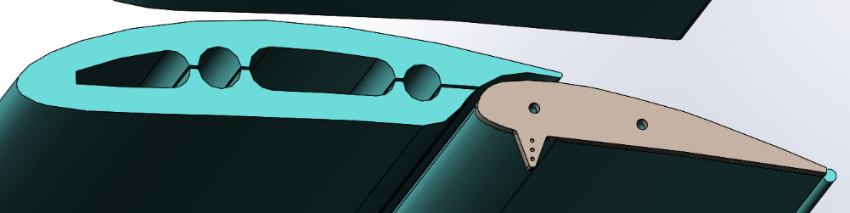
\includegraphics[width=\textwidth]{retracted-flap}
        \caption{Retracted}
        \label{fig:flaps:retracted}
    \end{subfigure}
    \hfill
    \begin{subfigure}[b]{0.49\columnwidth}
        \centering
        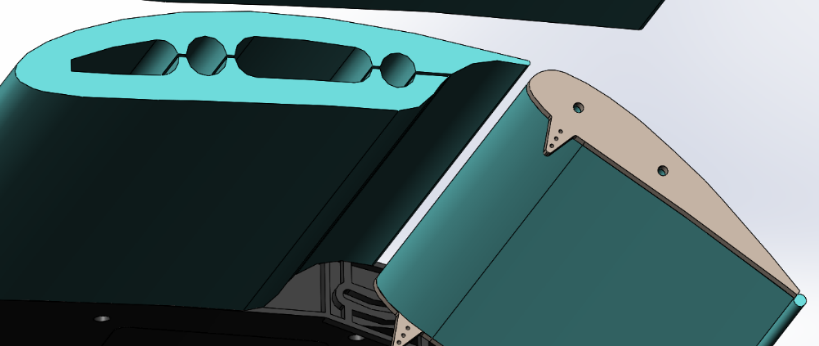
\includegraphics[width=\textwidth]{deployed-flap}
        \caption{Deployed}
        \label{fig:flaps:deployed}
    \end{subfigure}
    
    \caption{flap, with endplates for horn controls.}
    \label{fig:flaps}
\end{figure}

\section{Fuselage} \label{sec:final-design-proposal:fuselage}

\subsection{Central structure} \label{sec:final-design-proposal:fuselage:central-structure}

The main focus for the design of the UAV's fuselage was to provide a reliable and simple platform for the experiments.
The concept for the design of the fuselage revolved around the idea of providing easy access to the electronics.
Changing the motor configuration multiple times demands the ability to check and modify the electronics with ease in order to proceed with the experiments in a smooth manner.
The design therefore presents a large electronics tray placed in the lower section of the fuselage, shown in purple in Figure \ref{fig:fuselage-inner-structure}.
This can be accessed through the removal of the UAV's nose.

\importimage{fuselage-inner-structure}{CAD representation of the inner structure of the fuselage's central section.}{Fuselage inner structure}{0.8}

All of the fuselage's structural components are located in the top section of this part.
In so doing a large area was created for the housing of the electronics as shown in Figure \ref{fig:fuselage-inner-structure}.
The supports for the electronics tray, also referred as the fuselage ribs, were designed to be manufactured out of \mm{5} birch wood sheets.
Such supports (shown in brown in Figure \ref{fig:fuselage-inner-structure}) are mounted onto the fuselage central beam.
This is a square section carbon spar (\mm{20} $\times$ \mm{20}) which extends for the entire fuselage length. 

A carbon fibre sandwich panel is placed onto the top surface of the fuselage's central spar.
This is bonded at the wing's attachment area with the aid of epoxy bonding agent.
Its function is to provide the four mounting points for the bolts so as to allow the fixing of the wing assembly to the fuselage.
The sandwich panel is comprised of a \mm{5} thick nomex core placed between two carbon skins.
These are each made out of three ply woven carbon prepreg cured in autoclave.
Mounted below the plate are two PLA printed brackets (Figure \ref{fig:pla-bracket}); these are responsible for the correct positioning of the fuselage ribs and the landing gear mounting structure (Figure \ref{fig:brackets-highlighted}).
Furthermore, they are designed to withstand a vertical load of \newtons{170} each, thus offering a redundant attachment for the mounting plate in case of failure.

\importimage{pla-bracket}{CAD representation of the PLA bracket.}{PLA bracket}{0.5}
\importimage{brackets-highlighted}{fuselage central assembly with brackets highlighted in green.}{Highlighted brackets}{0.7}

\subsection{Landing gear attachment} \label{sec:final-design-proposal:fuselage:landing-gear-attachment}

The aircraft was designed to not exceed \kg{7} of total mass.
Hence the position and the mass of the landing gear structure proved to be of significance in positioning the aircraft's centre of gravity.
Its ideal position was set to be at \pc{50} of the wing's chord length, with a \pc{5} shift caused by the change in propulsion configuration.
The landing gear is mounted on two C-shaped \mm{5} aluminium brackets.
These are mounted to two bulkheads as shown in Figure \ref{fig:landing-gear-attachment}, and fulfil the role of transferring and absorbing the vertical loads encountered during taxi, takeoff, and landing.
In order to minimise the weight of this structure the bulkheads were designed to be manufactured as carbon fibre sandwich panels.
These have been specified to withstand vertical loads up to $5g$.
Furthermore, two triangular braces, as shown in Figure \ref{fig:landing-gear-attachment:side}, are attached to the lowest section of the bulkheads and are clamped to the main spar through a PLA insert.
These work in compression and are designed to counteract the moments generated by the loads acting on the wheels in the direction of travel. 

% \importimage{landing-gear-attachment}{landing gear attachment structure.}{Landing gear attachment}{0.4}
% \importimage{landing-gear-side}{landing gear attachment side view.}{Landing gear attachment side view}{0.4}

\begin{figure}[H]

    \centering
    \begin{subfigure}[b]{0.4\columnwidth}
        \centering
        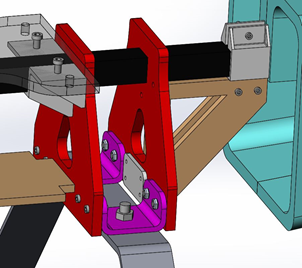
\includegraphics[width=\textwidth]{landing-gear-attachment}
        \caption{}
        \label{fig:landing-gear-attachment:angled}
    \end{subfigure}
    \hfill
    \begin{subfigure}[b]{0.49\columnwidth}
        \centering
        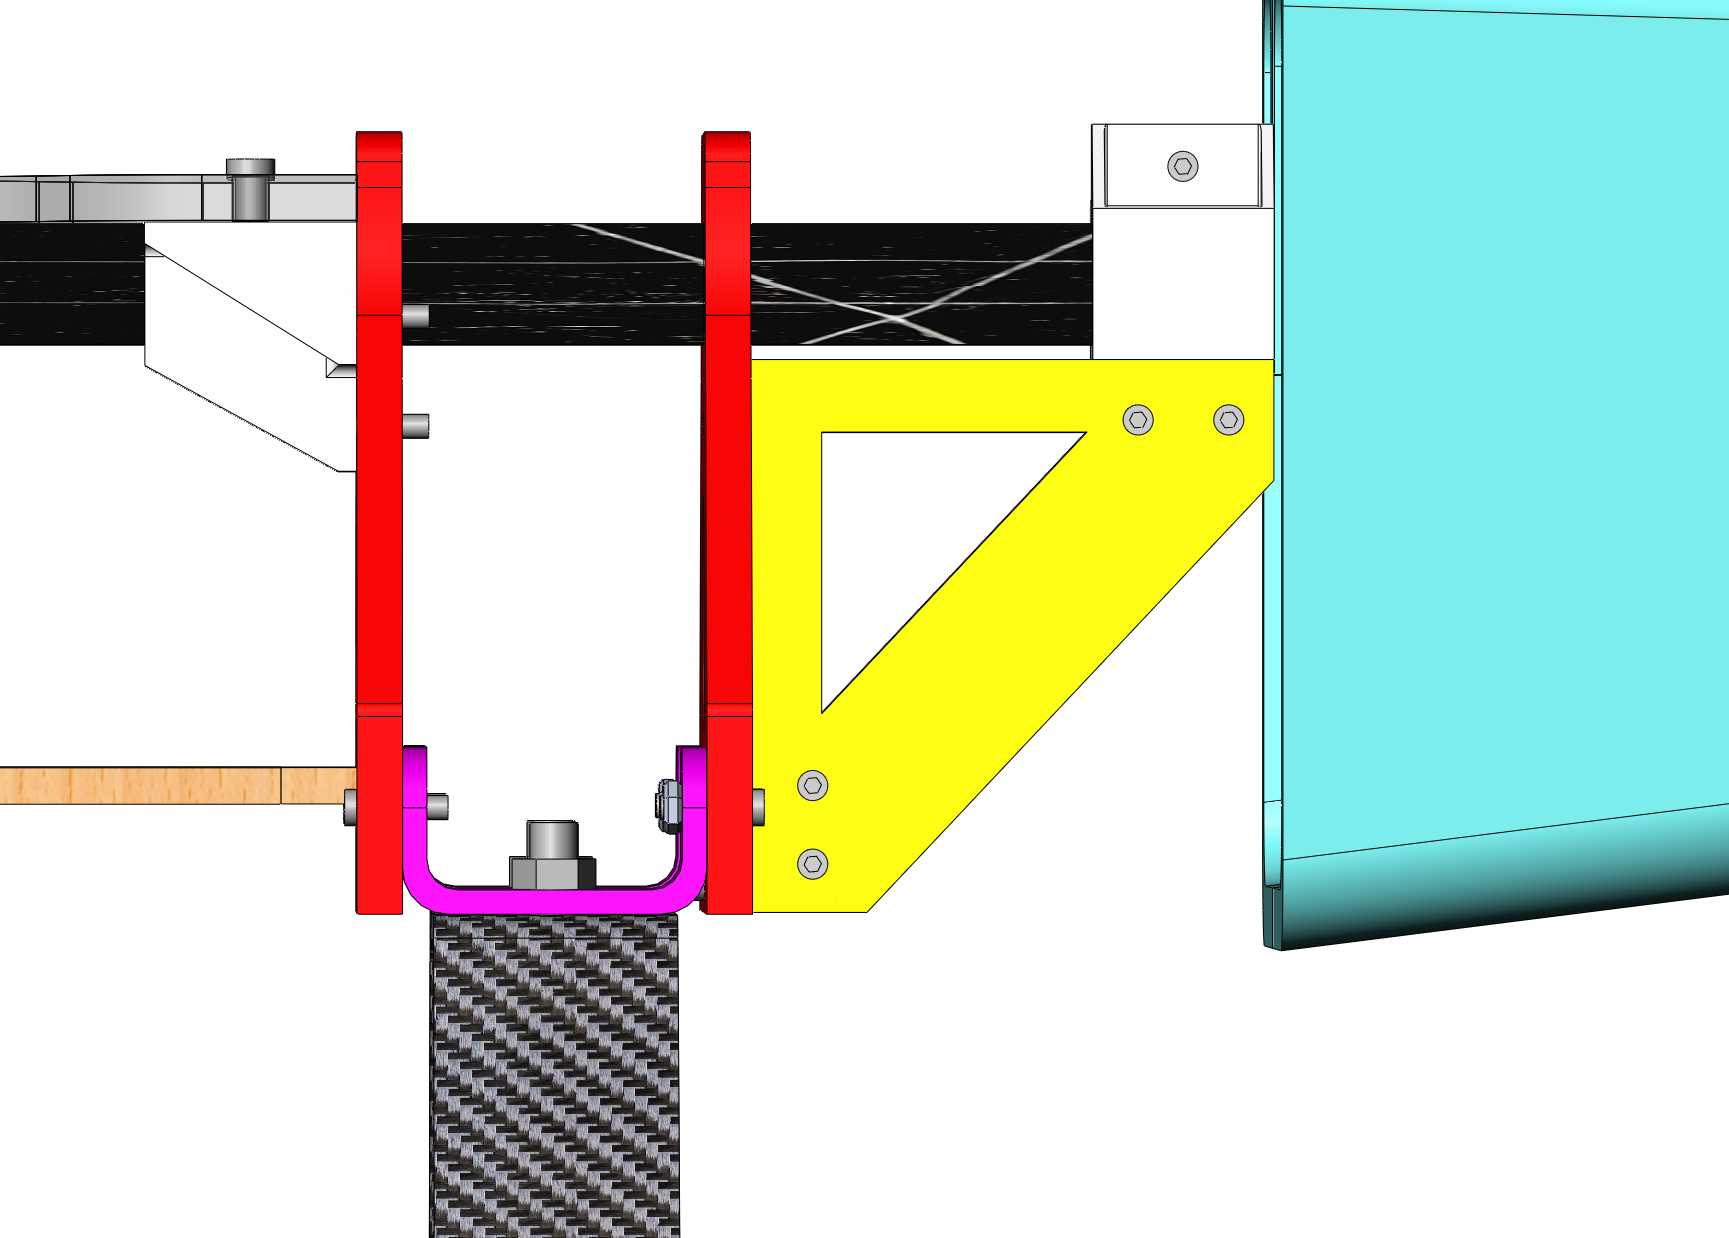
\includegraphics[width=\textwidth]{landing-gear-side}
        \caption{}
        \label{fig:landing-gear-attachment:side}
    \end{subfigure}
    
    \caption{landing gear attachment structure.}
    \label{fig:landing-gear-attachment}
\end{figure}

The carbon fibre sandwich panels bulkheads were designed in the same manner as the aforementioned fuselage central plate, whose schematic can be seen in Figure \ref{fig:carbon-fibre-sandwich}. 

\importimage{carbon-fibre-sandwich}{CAD representation of the carbon fibre sandwich panel components.}{Carbon fibre sandwich}{0.5}

\subsection{Finite element analysis} \label{sec:final-design-proposal:fuselage:finite-element-analysis}

In order to verify the strength of the design and identify any weak points, some FEA was carried out using the simulation function in SolidWorks.
This is a fairly basic FEA system and can only use coarse meshes $-$ otherwise the simulations fail $-$ but it gives a good indication of the strong and weak areas of the fuselage design.
The materials of the parts of the fuselage were all specified and the data for those materials applied as accurately as possible in order to ensure the parts' relative strengths were reflected in the simulations.
The model was stripped down to the minimum components required to perform the simulations in order to save computational time and simplify the simulations.
Initially a simulation was run to test the effects of high turning loads, with the main tail boom fixed in place as the reference point of the study, with loads of \newtons{210} applied vertically upwards on the wing spar holes in the wing mount, and \newtons{80} applied vertically down on the component tray.
These loads were chosen to simulate $3g$ loads in a turn, with the mass of the components assumed to be evenly distributed over the tray.
Figure \ref{fig:fuselage-stress-distribution} shows the results.

\importimage{fuselage-stress-distribution}{fuselage stress distribution during a simulated $3g$ turn.}{Fuselage stress distribution}{0.7}

It can be seen that the wing mount shows that the maximum stress experienced is around 1.6 MPa, which is significantly below the 30 MPa yield stress of the ABS material used.
The other high stress locations are on the lower parts of the component tray mounts, which peak at over 2 MPa, but the plywood used has a yield stress of 30 MPa and so this is also well below the point of breaking.
It can also be seen that the stress on the carbon fibre tail boom reaches over 2 MPa, but this is well below the yield stress of the carbon tube which will be over 600 MPa based on the properties quoted at \cite{unknown}. % TODO: [Performance Composites [REF]]. 

The second simulation determined the effects of landing loads, with the tail boom again fixed and the loads applied at the locations of the wheel centres on the landing gear.
This simulation only tested the main gear as this is where the highest forces should be experienced if the UAV is landed properly.
The forces applied are \newtons{350} vertically up and \newtons{105} horizontally backwards to simulate a heavy landing of $5g$ with $1.5g$ deceleration force. 

\importimage{landing-leg-simulation}{simulated stress distribution over one of the landing legs.}{Landing leg simulation}{0.4}
\importimage{fuselage-landing-simulation}{stress distribution over the fuselage during a simulated landing.}{Fuselage landing simulation}{0.6}

It can be seen in Figure \ref{fig:landing-leg-simulaion} that the peak loads experienced by the landing gear are around 260 MPa, which is below the yield stress of the carbon fibre as previously stated, and although it is nearing the yield stress, this is an extreme case of a particularly heavy landing and so a heavier landing than this would not be expected unless it occurs in a crash landing scenario (in which case the UAV's survival can never be guaranteed).
It can also be seen that the peak stress on the landing gear brackets is around 100 MPa, below the yield stress of around 270 MPa of the aluminium from which they are made.
With the scale modified to a reduced upper bound, the stresses on the other parts can be seen, with the peak stress experienced by the landing gear mounts seen as around 10 MPa, which is far below the yield stress of carbon fibre and so $-$ although the properties of carbon fibre sandwich panel are varied $-$ this is not close to failure. 

\section{Landing gear} \label{sec:final-design-proposal:landing-gear}

% TODO: could this go under design process?

Two main types of landing gear design were considered for this project: the tricycle and a tail wheel approach.
A tricycle consists of a single front wheel, and two rear wheels, as seen on most commercial aircraft; whereas a tail wheel design uses a single rear wheel with two front wheels.

\importtable{| >{\raggedright\arraybackslash}p{0.12\columnwidth} | >{\raggedright\arraybackslash}p{0.36\columnwidth} | >{\raggedright\arraybackslash}p{0.36\columnwidth} |}{
    \hline
    \textbf{Design} & \textbf{Advantages} & \textbf{Disadvantages} \\
    \hline
    Tricycle & Prevents nose tipping; improved stability; better manoeuvrability; better in crosswinds & Increased drag and weight; nose gears are prone to damage \\
    \hline
    Tail wheel & Lighter; easier to integrate with under rudder; more suitable for integration with nose design; propellors would have more ground clearance & Harder to attach front wheels; harder to manoeuvre \\
    \hline
}{tradeoffs involved in the gear layout used.}{gear-layout-tradeoffs}

When the landing gear was first being designed weight was the limiting factor, with the UAV close to the \kg{7} mass limit.
Because of this the decision was made to use a tail wheel approach as it is lighter than the tricycle approach.
The modularity and moving centre of gravity was a challenge unique challenge to this UAV, however, and the first step of the design was the calculation of the maximum loading conditions the landing gear would encounter \cite{goud-14}. 

\importimage{moment-calculations}{moment calculations.}{Moment calculations}{0.7}

The forwardmost centre of gravity (CG) meant $x=150\,\mathrm{mm}$ and $y=765\,\mathrm{mm}$, which led to a maximum static loading of \newtons{57.4} over the front wheels and \newtons{11.26} over the rear wheel.
The rearmost CG led to $x=200\,\mathrm{mm}$ and $y=815\,\mathrm{mm}$; the maximum static loadings for this condition are \newtons{55.13} and \newtons{13.53} over the front and rear wheels respectively.
Based on these calculations, a load of \newtons{57.4} and \newtons{13.53} were used in future calculations and analyses. 

A vertical velocity of \mps{3} was assumed to be an aggressive landing velocity in the hands of a competent pilot and so was used in calculation to ensure the landing gear would be strong enough to withstand multiple rough landings.
Using Newton's $2^\mathrm{nd}$ law, and an assumed impact time of 0.5 seconds, the maximum force of the UAV would be equal to \newtons{42}, meaning a total force of \newtons{110.67} on landing.
Since most UAVs land with their main wheels touching down first, the main landing gear must absorb the majority of the load: from previous calculations, the main gear should withstand \newtons{99.4}.  

\importimage{landing-gear-design-one}{landing gear design one.}{Landing gear design}{0.8}

A setting angle of \degr{5.8} was needed to meet takeoff requirements, as shown in Figure \ref{fig:landing-gear-design-one}.
To avoid hitting the rear propeller or the rudder, the rear wheel was designed to extrude from the bottom of the under-rudder.
The carbon fibre spar in the rudder would be strong enough to support the maximum \newtons{10} load it would encounter on landing. 

\importimage{landing-gear-attachment-locations}{potential landing gear attachment locations.}{Landing gear attachment locations}{0.7}

It immediately became clear that the main gear would have to be mounted to the main carbon fibre boom running the length of the fuselage.
Following advice from the project supervisor, however, it was decided that the main wheels should be located below the leading edge of the wing.
As Figure \ref{fig:landing-gear-attachment-locations} shows, mounting the main gear would not be possible in this location.
A solution involving having the main gear mounted further forward but curved backwards was investigated.  

Several iterations similar to the final design in Figure \ref{fig:main-gear-progression:final} were designed and tested using FEA.
The FEA was initially carried out on a single leg, with a loading of \newtons{50} applied to a fiberglass construction.
After the design of the leg was finalised a clamping system was devised to mount the main gear to the boom.
Further FEA showed that the clamping would be effective at attaching the fibreglass to the boom but would cause the boom to buckle on landing.
Figure \ref{fig:prepreg-cover-stress} shows how the addition of a prepreg cover around the boom significantly reduces the stress of the boom itself, roughly by a factor of 10. 

% \importimage{landing-gear-design}{main landing gear design.}{Landing gear design}{0.4}
\importimage{landing-gear-stress}{stress on landing gear.}{Landing gear stress}{0.5}
\importimage{prepreg-cover-stress}{effect of a prepreg cover on carbon fibre spar.}{Prepreg cover stress}{0.95}

At this point in the design process, the weight of the UAV was no longer an issue, and after a supervisor meeting in which the landing gear design was discussed it was decided that the landing gear should be steerable.
This would reduce the time taken time to retrieve the UAV upon landing as well as making takeoff easier.
The tail wheel setup is not optimal for a steerable configuration and so, as the fuselage and the weight of the aircraft had been reduced $-$ making weight less of a limiting factor $-$ the decision was made to redesign the landing gear in a tricycle configuration. 
FEA was carried out on the design and small changes were made until an optimal design was found.

\begin{figure}[H]
    \centering
    \begin{subfigure}[b]{0.33\columnwidth}
        \centering
        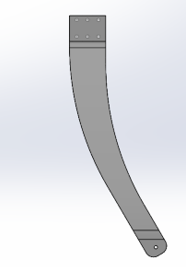
\includegraphics[width=\textwidth]{landing-gear-design}
        \caption{Initial}
        \label{fig:main-gear-progression:initial}
    \end{subfigure}
    \hfill
    \begin{subfigure}[b]{0.49\columnwidth}
        \centering
        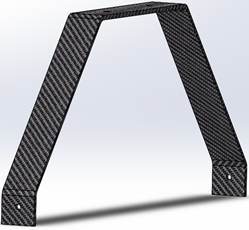
\includegraphics[width=\textwidth]{main-gear-design}
        \caption{Final}
        \label{fig:main-gear-progression:final}
    \end{subfigure}
    
    \caption{progression of the main gear design.}
    \label{fig:main-gear-progression}
\end{figure}

% TODO: start final design proposal section for gear here?

Using a similar process to that used in the original tail wheel design, it was calculated that the main landing gear would experience up to \newtons{105.8} on landing.  % TODO: add section reference if reordered
The main gear in the final design proposal is located behind the centre of gravity, behind the internal electronics.
This, along with a redesigned fuselage means the landing gear could be designed as a single part and attached easily to the bottom of the fuselage. 

% \importimage{main-gear-design}{main gear design.}{Main gear design}{0.4}
\importimage{main-gear-fea}{main gear FEA stress results.}{Main gear FEA}{0.6}

The main shape of the design remains unchanged from the initial design, and is a similar design to that seen on many small UAVs which is simple, easy to implement, and robust.
The final design is expected to experience a maximum stress of 92.5 MPa on a rough landing, and is manufactured from carbon fibre because it can be manufactured cheaply in university workshops and has a high strength to weight ratio.
The final design has a maximum thickness of \mm{6} at the top where it joins the fuselage, narrowing to \mm{4} by the wheels.
The depth remained constant at \mm{65}, with a wheelbase of \mm{490} and a height of \mm{220} to avoid hitting the under-rudder on takeoff.
The redesigned fuselage structure with two lower plates means that the landing gear can easily be mounted to the fuselage using two M4 bolts. 

Eventually, a landing gear model very similar to the one described here was found online and purchased instead of manufacturing one from scratch; this was found to be more time- and cost-effective.

\importimage{landing-gear-join}{landing gear joining mechanism.}{Landing gear joining mechanism}{0.6}

The nose gear was chosen at the recommendation of the project co-supervisor and is the same as the one used on the SPOTTER aircraft \cite{spotter-19}, a \kg{24} split fuselage UAV.
It is easy to implement into the nose and is steerable, while also being cheap, lightweight, and strong. 

\section{Nose} \label{sec:final-design-proposal:nose}

% TODO: split part of this into the design process section

The nose was a key component in the project and needed to fulfil several criteria:

\begin{itemize}
    \item support a motor and propellor unit;
    \item provide access to the motor for removal;
    \item be removable from the rest of the fuselage whilst being strong enough to support the motor during flight;
    \item integrate the landing gear.
\end{itemize}

To fulfil all the above criteria, it was obvious from the start that the nose would have to be 3D printed, meaning there were no geometry restrictions placed upon the design. 
The initial design was simple, incorporating the ability to attach the motor via four internal screw holes.
The nose would be attached to the fuselage via a spar running through the nose and the front of the spar.
Although not optimal, at the time it was deemed acceptable to drill through the end of the carbon spar as it was away from the structural core of the fuselage.
The design also incorporated a slot for the battery to slide into to act as a ballast, as well as a slot for the ESC, which would maximise airflow to it for cooling purposes.

\begin{figure}[H]
    \centering
    \begin{subfigure}[b]{0.6\columnwidth}
        \centering
        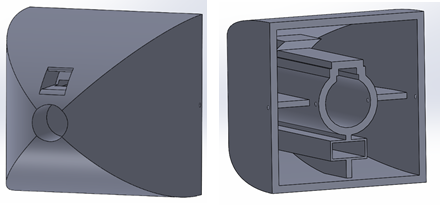
\includegraphics[width=\textwidth]{initial-nose-design}
        \caption{Initial}
        \label{fig:nose-design-progression:initial}
    \end{subfigure}
    
    \begin{subfigure}[b]{0.6\columnwidth}
        \centering
        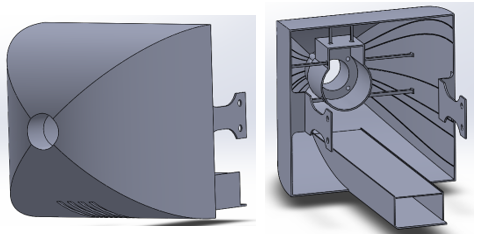
\includegraphics[width=\textwidth]{revised-nose-design}
        \caption{Revised}
        \label{fig:nose-design-progression:revised}
    \end{subfigure}

    \begin{subfigure}[b]{0.6\columnwidth}
        \centering
        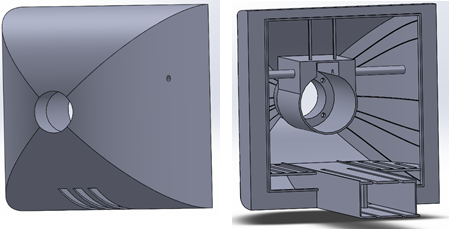
\includegraphics[width=\textwidth]{twice-revised-nose}
        \caption{Final}
        \label{fig:nose-design-progression:final}
    \end{subfigure}
    
    \caption{various stages of the design of the printed nose.}
    \label{fig:nose-design-progression}
\end{figure} 

% \importimage{initial-nose-design}{initial nose design.}{Initial nose design}{0.6}

Figure \ref{fig:nose-design-progression:revised} shows an updated version of the nose design.
Firstly, the outer body was lightweighted considerably from \mm{5} to \mm{1.5}, and supports were added.
The battery compartment became a tray, which will serves to make removal easier.
The tray had a section underneath in which the ESC was to be placed, with cooling vents in the front of the nose.
The nose was to be secured to the fuselage via two bolts along the width of the fuselage.
More light weighting was done to the motor support and rods used in place of the previous bulky design. 

% \importimage{revised-nose-design}{revised nose design.}{Revised nose design}{0.7}

After advice from the project supervisor, alterations were made to the revised design.
Most notably, a battery and ESC tray were added to the back of the nose, with vents in the front of the nose to allow cooling to the ESC.
The tray was supported by two vertical poles to support the weight of the battery. 

% \importimage{twice-revised-nose}{twice revised nose design.}{Twice revised nose design}{0.7}

The nose would now be secured by one bolt, through the carbon fibre spar, which would also act as a support for the motor mount.
After further deliberation with the project supervisor, however, it was decided that the loss in structural performance from drilling through the carbon fibre boom was not worth the reduction in workload, so a new way of attaching the nose to the fuselage was sought.  

The new multi-component nose design had two components.
The inner component would be secured to the fuselage at all times, and the front part would be removeable.
The inner part would be secured to the boom using a clamping mechanism, originally devised for the landing gear, via three M3 bolts located underneath the boom.
The outer part would then twist into the inner part and be locked in place using two M3 bolts. 

\begin{figure}[H]
    \centering
    \begin{subfigure}[b]{0.6\columnwidth}
        \centering
        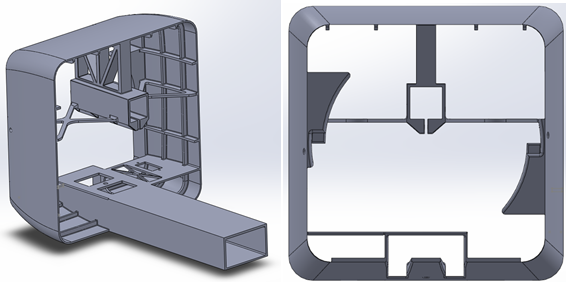
\includegraphics[width=\textwidth]{nose-inner-section}
        \caption{Inner section}
        \label{fig:nose-design:inner}
    \end{subfigure}
    
    \begin{subfigure}[b]{0.6\columnwidth}
        \centering
        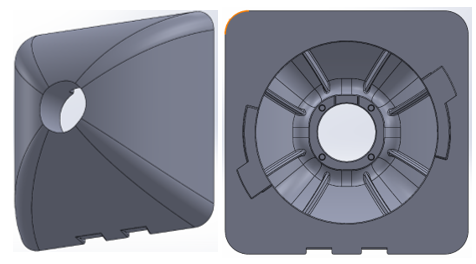
\includegraphics[width=\textwidth]{nose-outer-section}
        \caption{Outer section}
        \label{fig:nose-design:outer}
    \end{subfigure}

    \begin{subfigure}[b]{0.6\columnwidth}
        \centering
        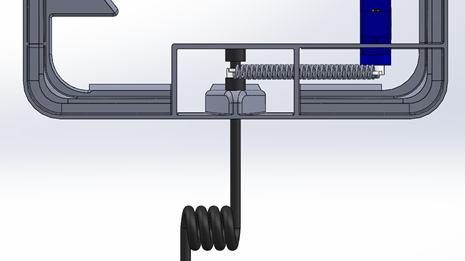
\includegraphics[width=\textwidth]{steerable-gear}
        \caption{Steerable gear attachment}
        \label{fig:nose-design:steerable-nose-gear}
    \end{subfigure}
    
    \caption{detailed models of the final nose design.}
    \label{fig:nose-design}
\end{figure} 

% \importimage{nose-inner-section}{inner section of the nose.}{Nose inner section}{0.7}

The inner part would had a \mm{1} wall thickness, supported by \mm{5} deep and \mm{3} wide support structures common on 3D printed UAV components as they are such a light way of increasing strength.
The clamping system was supported by a web-like structure.
The battery tray and ESC compartment were given a small redesign, with two larger vents channelling airflow to the ESC.
The steerable landing gear were also incorporated into the design, through the air vents. 

% \importimage{nose-outer-section}{outer section of the nose.}{Nose outer section}{0.7}

The outer section would be held in place via a twist and lock system.
To remove the front section, two screws would be removed from the side of the nose; the front would then twist anticlockwise and be removed.
Once removed, the electronics inside could be easily removed over the battery tray.
The motor could easily be removed via four screws located towards the front of the nose and replaced by a 3D printed part for aerodynamic purposes when the nose motor is not in use.
The motor mount area was also lightened, with similar structural supports on the \mm{1} outer wall. 

\importimage{outer-nose-fea}{FEA on the outer nose join.}{Nose join FEA}{0.7}

FEA was carried out on the outer section to ensure it was strong enough to support the fuselage.
Figure \ref{fig:outer-nose-fea} shows a \newtons{140} force applied to the locking tabs.
For SLS nylon the yield strength was set at 60 Mpa.
With the \newtons{140} load applied, however, the maximum stress reached was 5.582 MPa, resulting in a maximum displacement of \mm{0.1}. 

% TODO: move to final design proposal here?

The final design of the nose also incorporates a steerable landing gear.
This part of the design was carefully considered throughout the design process, but only fully implemented after the landing gear design had been finalised. 

% \importimage{steerable-gear}{integration of the steerable nose gear.}{Steerable nose gear}{0.7}

Figure \ref{fig:nose-design:steerable-nose-gear} shows how the nose gear is incorporated within the vent design.
The nose gear is secured using two collars, one above and one below the thicker part of the nose, as well as one to secure the servo arm in place.
The servo arm is attached to the servo via two springs, which alleviate impacts and prevent the nose from rapid direction changes due to bumps.
The servo is bolted onto the battery tray, to one side, to allow space for the battery tray to be removed. 

As mentioned during the analysis of the landing gear, depending on the configuration, the landing gear will have to withstand a force of up to around \newtons{35} on landing.
Therefore, further FEA was carried out on the nose.
The results (Figure \ref{fig:nose-connection-fea}) show a moderate level of stress on the wall at the bottom of the vent, although this was about half of the perceived yield strength of the SLS nylon which is to be used. 

\importimage{nose-connection-fea}{FEA on nose and landing gear connection.}{Nose connection FEA}{0.7}

When the nose motor is not needed it can be removed and replaced with a small insert.
The hollow insert is to be 3D printed on the university 3D printer using PLA as it is not a structural component.
It was designed to be screwed in in the same manner as the motor. 

\importimage{nose-motor-filler}{nose motor filler.}{Nose motor filler}{0.5}

\section{Tail} \label{sec:final-design-proposal:tail}

\subsection{Mathematical modelling} \label{sec:final-design-proposal:tail:mathematical-modelling}

% TODO: move this to section on revised designs

The tail is required to provide adequate stability to the aircraft in all stages of flight, as well as house the elevator and rudder control surfaces.
Design for the tail and stability systems was restarted following research and dialogue with the project supervisors after the wind tunnel test, which revealed the true scope of the design process required. 

Revision began with the tail surfaces themselves.
As the centre of gravity of the aircraft would not be in line with the centre of lift, the tailplane would need an angle of attack that would facilitate the aircraft's stability throughout flight, with minimal to no trim from the elevators.
The sizing of the tail surfaces and their angles were again determined using processes described by Sadraey \cite{sadraey-13}.
In particular an example of tail design was followed from \S 6.1 (and slightly modified) to obtain the tail dimensions and setting angle. 

The process began similarly to that of the wind tunnel model.
Revised volume coefficients were suggested as 0.8 for the horizontal tail, and 0.06 for the vertical tail \cite{towell-19}.
The tail planform area was determined as $0.16 \mathrm{m^2}$ for the horizontal tail, and $0.08 \mathrm{m^2}$ for the vertical tail.  % TODO: work out where these equations went (originally [1] and [2])

Next, the cruise lift coefficient was determined, using equation 6.27 from \cite{sadraey-13}, and was found to be 0.4671, based on a weight of \kg{7} (\newtons{68/67}), cruise speed of \mps{20}, and wing planform area of $0.6 \mathrm{m^2}$.
The wing/fuselage aerodynamic pitching moment coefficient then needed to be estimated.
Sadraey provided an equation for this, but at the suggestion of the project supervisor, equation E-40 $-$ which determined the change in wing pitching moment due to the fuselage $-$ from E. Torenbeek’s book \cite{torenbeek-76} was used instead.
This was determined to be $-0.0398$.
Based on a chart from 'Airfoil Tools' for the NACA6412 aerofoil, the wing 0 lift pitching moment coefficient was determined to be -0.137 \cite{airfoil-tools-19}.
This and the fuselage offset were then summed to give a value of the wing/fuselage pitch moment coefficient of $-0.1768.$ 

The next stage of the process required values for the centre of lift and mass locations in terms of percent of the MAC of the wing.
As these were unknown at this stage, they were estimated to be $h = 0.25$ (quarter chord) for the centre of lift (a reasonable assumption for most wings) and $h_0 = 0.5$ (half chord) for the centre of mass, which was a worst case value. 

Next, the required lift coefficient of the horizontal tailplane needed to be determined.
Essentially, the moment caused by the lift, thrust and weight, as well as the wing pitching moment, has to be counteracted by a moment provided by the tail.
It was decided that this should be negated at the cruise speed of the UAV, reducing the work required by the pilot for the majority of the flight.
The tail uses a symmetrical aerofoil, and as such provides no lift force at \degr{0} incidence, so requires a mounting angle to provide a balancing moment.
This has to take into account changes to flow incidence caused by the fuselage angle of attack at cruise to make the wing provide sufficient weight, balancing lift $-$ as well as flow downwash $-$ caused by the wing. 

To calculate the tail cruise lift coefficient, equation 6.29 from Sadraey \cite{sadraey-13} could be used; the project supervisor, however, suggested a method which rearranged a substituted force and moment balance of the aircraft in cruise, which resulted in an equation for the angle of attack of the fuselage relative to the wing zero lift line: 

\importequation{
    \alpha_{F_{0L}} = \frac{
        \frac{2mg}{V^2} + \frac{C_{m0}c}{l}
    }{
        \rho S C_{L\alpha} (1 + \frac{h-h_0}{l})
    }
}{tail-cruise-lift-coefficient}

At \mps{20}, the fuselage angle was determined to be 0.0944 radians (relative to wing zero lift).
The tail cruise lift coefficient could then be determined using a modified version of equation 6.29 from Sadraey \cite{sadraey-13} as $-0.0871$.
Using an equation for the lift coefficient $C_\mathrm{L} = C_{L\alpha}\alpha$, the required incidence of the tail could then be determined as \degr{-1.238}.  % TODO: add mathrm inside $
The fuselage angle of attack had been determined relative to the wing zero lift line previously.
The wing zero lift line was \degr{5.7}, and the wing was mounted at \degr{2}, giving the wing zero lift line as \degr{7.7} relative to the fuselage datum.
This gave the fuselage angle of attack in flight as \degr{-2.294}.  

The wing downwash calculation required the downwash at zero angle of attack, and the downwash curve slope.
These were both determined using equation E-52 in \cite{torenbeek-76}: calculating these values and substituting into the equation for downwash gave a value for the downwash caused by the wing, at the tail as \degr{1.924}.
Finally, the tail setting angle could be calculated, which resulted in a setting angle relative to the fuselage datum of \degr{2.979}. 

% \importimage{resulting-tail-design}{the resulting tail design.}{Resulting tail design}{0.4}
% \importimage{resulting-tail-design-side}{the resulting tail design, viewed from the side.}{Resulting tail design side}{0.4}

\begin{figure}[H]

    \centering
    \begin{subfigure}[b]{0.49\columnwidth}
        \centering
        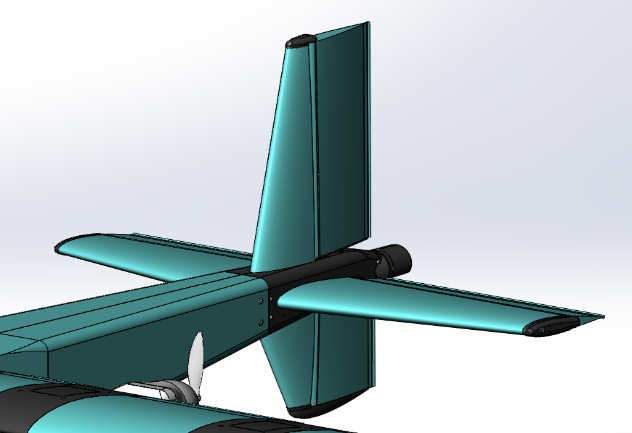
\includegraphics[width=\textwidth]{resulting-tail-design}
        \caption{}
        \label{fig:final-tail-design:angle}
    \end{subfigure}
    \hfill
    \begin{subfigure}[b]{0.49\columnwidth}
        \centering
        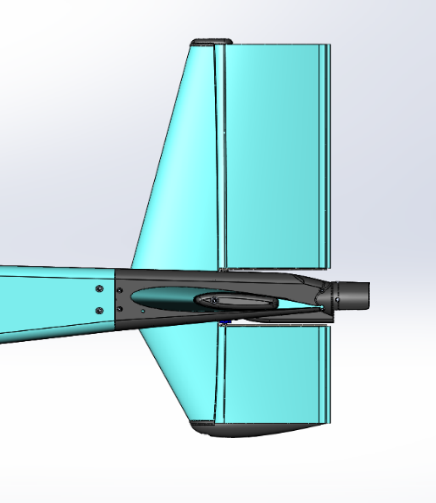
\includegraphics[width=\textwidth]{resulting-tail-design-side}
        \caption{}
        \label{fig:final-tail-design:side}
    \end{subfigure}
    
    \caption{resulting tail design.}
    \label{fig:final-tail-design}
\end{figure} 

One verification was to calculate the pitch stability derivative, using equation 6.67 in \cite{sadraey-13}, which resulted in $-0.6301$.
A negative value indicates that the pitch moment decreases with $\alpha$, which is desirable.
Following a process from \cite{de-kat-17} gave a stick fixed static margin of 0.1574, and a stick fixed manoeuvre margin of 0.2747, both of which are deemed to be acceptable values. 

Work on the yaw control requirements of the aircraft led to the decision to have an upper and lower vertical stabiliser, since extra rudder area was required, and to act as a bumper so that in the tail pusher propeller configuration $-$ where take off rotation or a hard landing might lead to tail propeller contacting the ground $-$ the propeller and therefore the aircraft would be protected.
Mounting a wheel on this bumper was considered when the UAV was planning use a tail wheel configuration, but when a nose wheel configuration was eventually settled upon, the bumper remained. 

Tail spars were resized using the same process as the wind tunnel model, as it had been decided to switch to pultruded carbon fibre rather than aluminium to save weight and move the centre of gravity forward.
The process does not account for the bonding of the extra foam material to the spars, so the estimated deflection would likely be pessimistic.  

Basic calculations from \cite{bresloff-18} were made to assess the potential effect of gusts and manoeuvres on tail loading.
It was estimated that the maximum load likely to be seen in a gust encounter at the predicted flight altitude was approximately \newtons{39}.
The maximum expected load from a manoeuvre was approximately \newtons{14}, both within the $10g$ limit load for which the aircraft was designed. 

\subsection{CAD modelling} \label{sec:final-design-proposal:tail:cad-modelling}

The tail surface CAD was generated as a lofted base using aerofoil profiles of a NACA0012 with a scaling factor applied to make a NACA0018, lining up at the trailing edge.
The root was shortened to allow for the tail mount geometry, and cutouts were added for the tail spars, control surfaces, and hot wire routes.
Initially the control surfaces were to be pinned into place with a laser cut sheet bonded to the end of the lifting surface holding a pin extending into control surface for it to rotate around, but in order to facilitate disassembly of the tail sub-assembly, this was changed into a 3D printed component that would neatly hold a nut on the end of a threaded rod bonded to the end of the tail spar.

The tail surfaces were designed to be inserted into 3D printed component as it was realised that the tail would require a lot of functionality that would be hard to facilitate with a foam or set of laser cut parts.
This was decided to be a piece that would split in half vertically, allowing the vertical surfaces to be inserted easily, and the horizontal surfaces would require a small amount of trimming to allow them to slide in over the spars, before being secured using bolts.
The CAD process for the final version of the tail mount can be seen in Figure \ref{fig:tail-mount-progression}.

% \importimage{tail-mount-one}{tail mount design, version one.}{Tail mount version one}{0.3}
% \importimage{tail-mount-two}{tail mount design, version two.}{Tail mount version two}{0.3}
% \importimage{tail-mount-three}{tail mount design, version three.}{Tail mount version three}{0.3}

\begin{figure}[H]
    \centering
    \begin{subfigure}[b]{0.32\columnwidth}
        \centering
        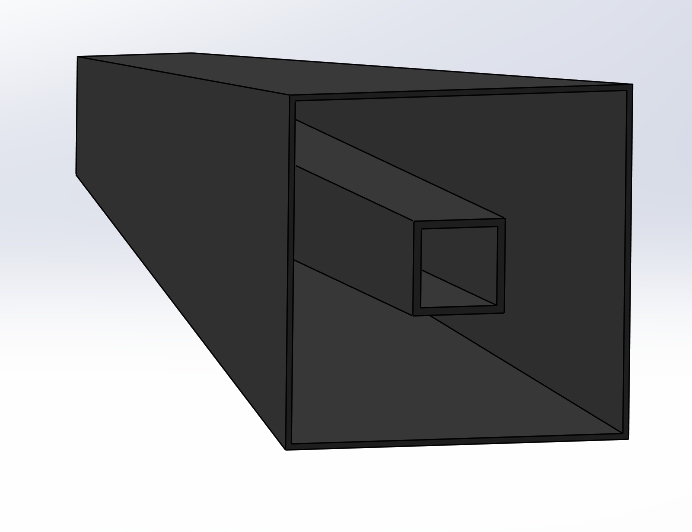
\includegraphics[width=\textwidth]{tail-mount-one}
        \caption{}
        \label{fig:tail-mount-progression:initial}
    \end{subfigure}
    \hfill
    \begin{subfigure}[b]{0.32\columnwidth}
        \centering
        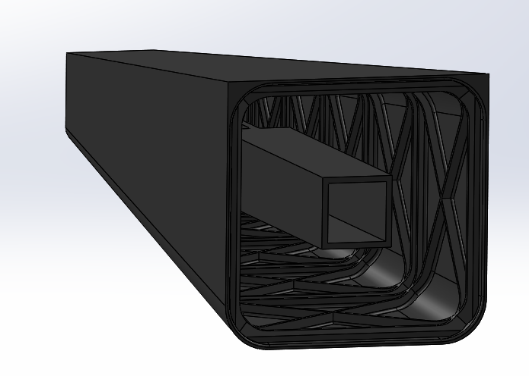
\includegraphics[width=\textwidth]{tail-mount-two}
        \caption{}
        \label{fig:tail-mount-progression:revised}
    \end{subfigure}
    \hfill
    \begin{subfigure}[b]{0.32\columnwidth}
        \centering
        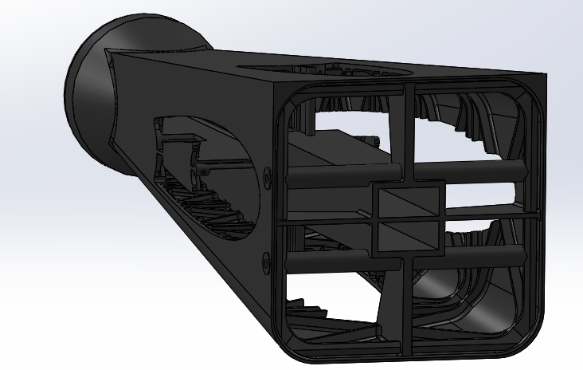
\includegraphics[width=\textwidth]{tail-mount-three}
        \caption{}
        \label{fig:tail-mount-progression:final}
    \end{subfigure}
    
    \caption{progressive iterations of the tail mount design.}
    \label{fig:tail-mount-progression}
\end{figure} 

% TODO: can this be turned into a section describing the final design rather than the CAD process?

The process began with a tapered section hollowed out to \mm{1.5} wall thickness, and a rectangular tube added for the tail spar.
The inside and outside corners were filleted. 
Next, ribs were added for lightweight structural support, made by a complex series of combined bodies.
Supporting structure was added from the outside walls to meet the spar tube in the centre.
A mounting location was added for the tail motor, and channels to run securing bolts through were added, as it was intended to make the part in two halves to aid assembly.  
In an assembly, the tail lifting surfaces were added, and moved to the correct position using mates, and then their bodies were subtracted from the mount body. 

Servo mounts were added and a motor mounting solution added based on a teammates previous design, and then a shroud was added over the motor, as well as a wire route for the motor connections.
The structure was eventually split in half and holes for spars added, and the model tidied up for 3D printing. 
A small structure was added to the front to allow for mounting to the foam ahead of it.

Finally, a small 3D printed part was designed to fit into the attachment location at the rear of the tail mount.
This was based on a prior design from earlier on in the project's design process, and simply had a cylinder with wide radial teeth protruding from the inside.
The motor mount had the same teeth, and would slide axially in the cylinder through the gaps, and then rotate, the teeth overlapping to prevent the mount from moving.
Small holes cut through both parts of the mount allowed for threaded inserts to be placed inside, and then screws through the same holes would secure the mount in place. 

% \importimage{tail-mount-slice}{a view of one half of the final tail mount.}{Tail mount slice}{0.4}
% \importimage{tail-mount-final}{a view of the final tail mount design.}{Tail mount design}{0.4}

\begin{figure}[H]
    \centering
    \begin{subfigure}[b]{0.49\columnwidth}
        \centering
        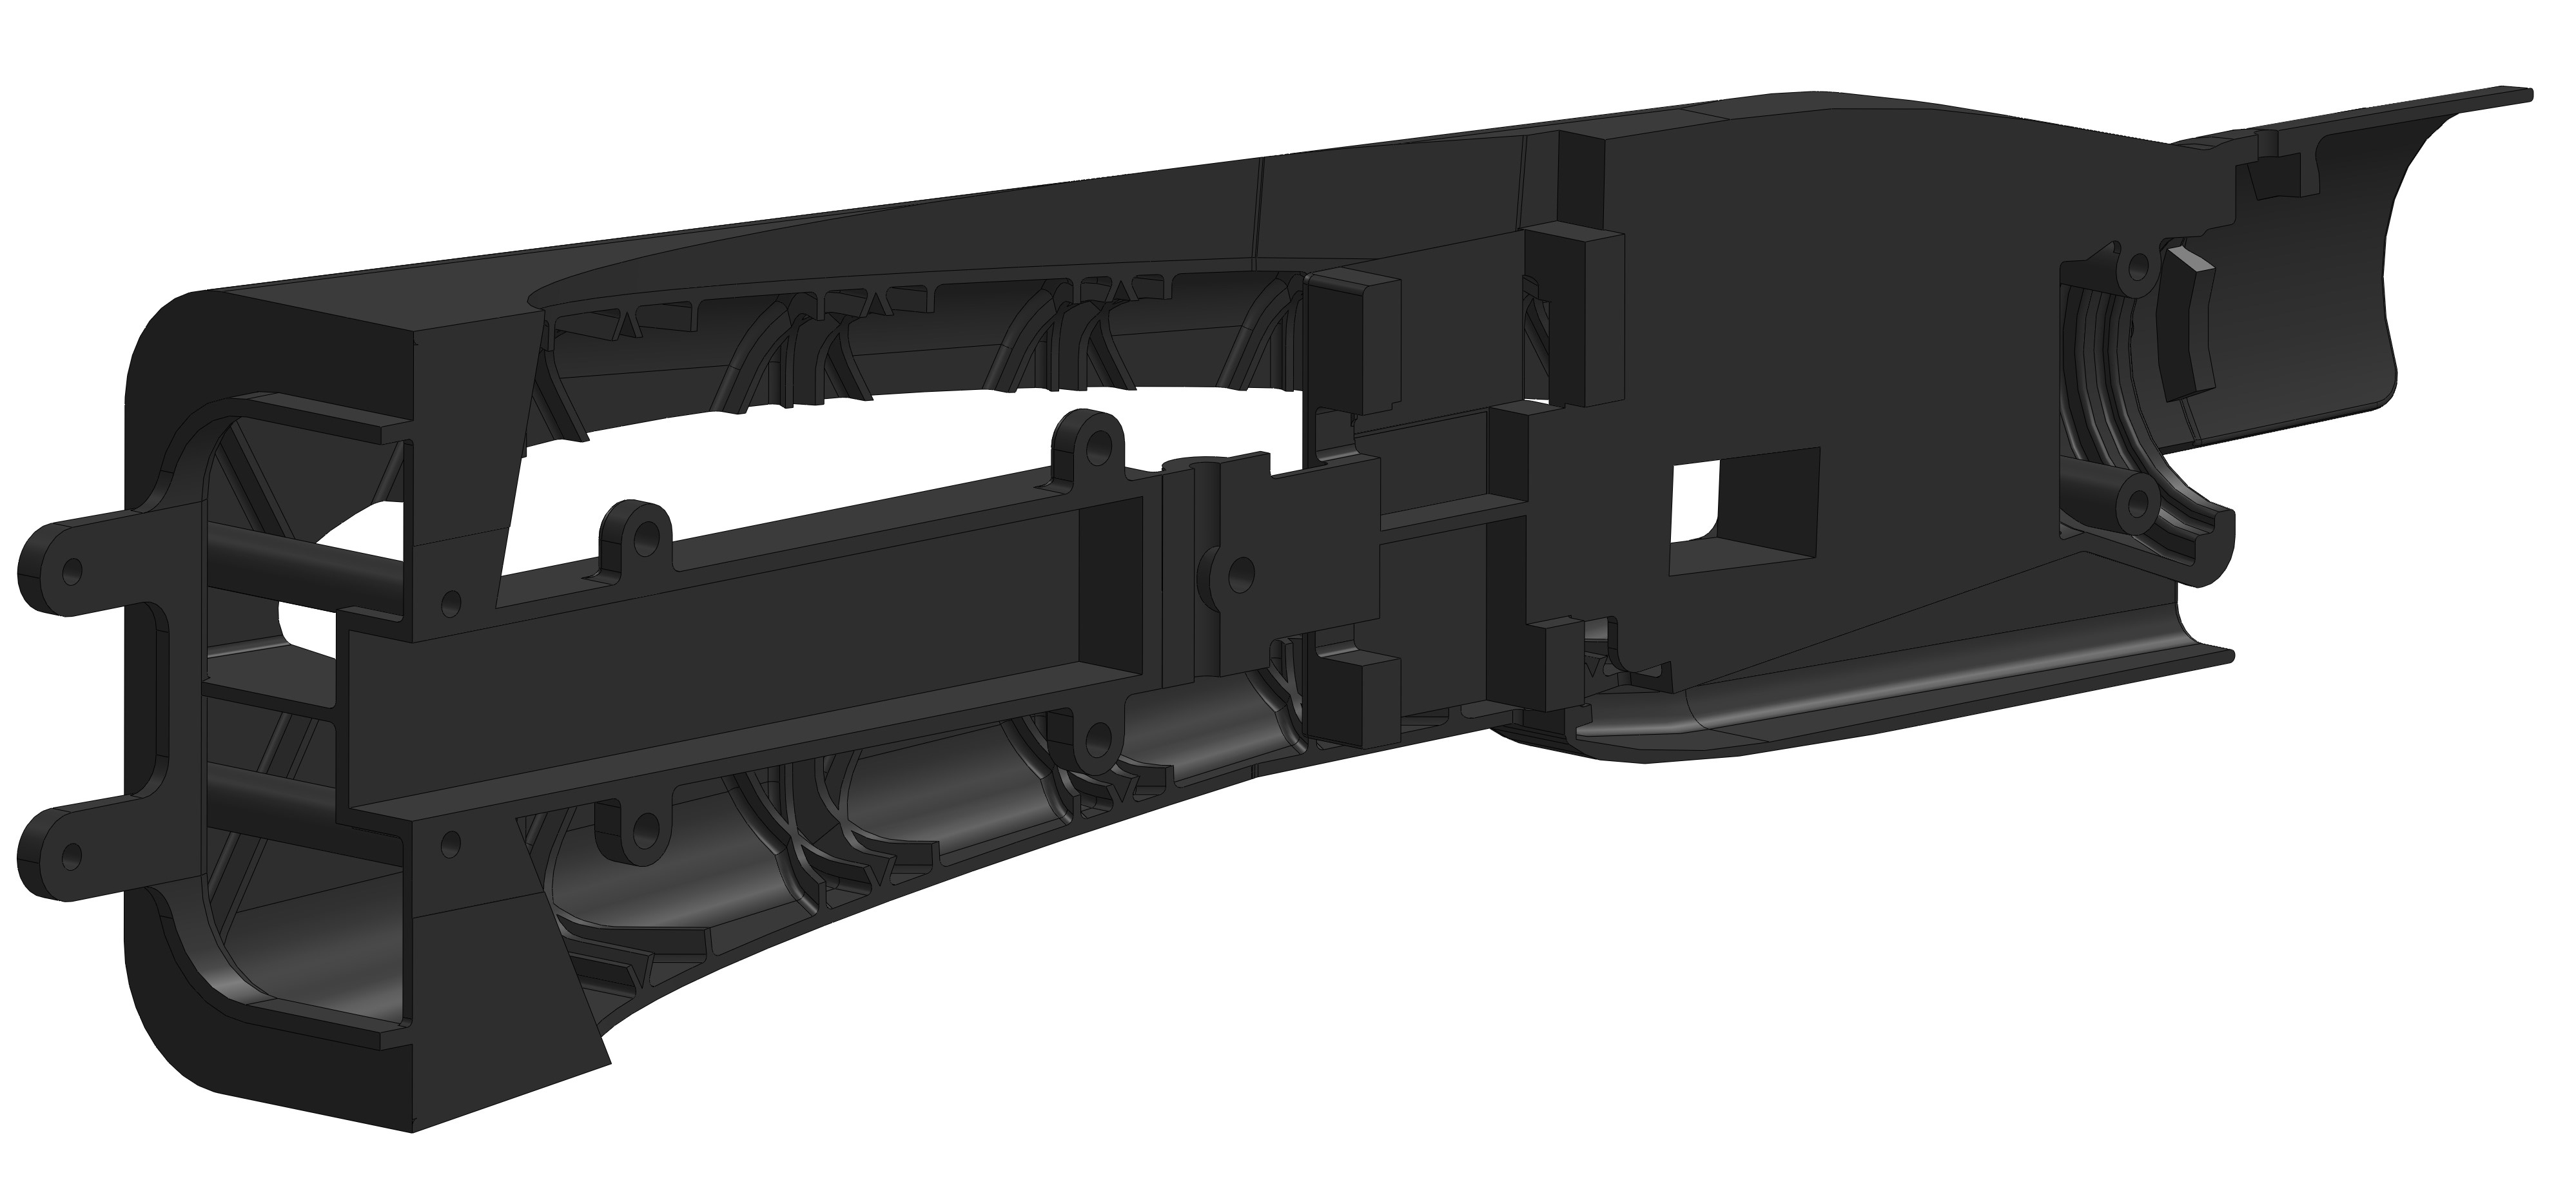
\includegraphics[width=\textwidth]{tail-mount-slice}
        \caption{}
        \label{fig:tail-mount-design:slice}
    \end{subfigure}
    \hfill
    \begin{subfigure}[b]{0.49\columnwidth}
        \centering
        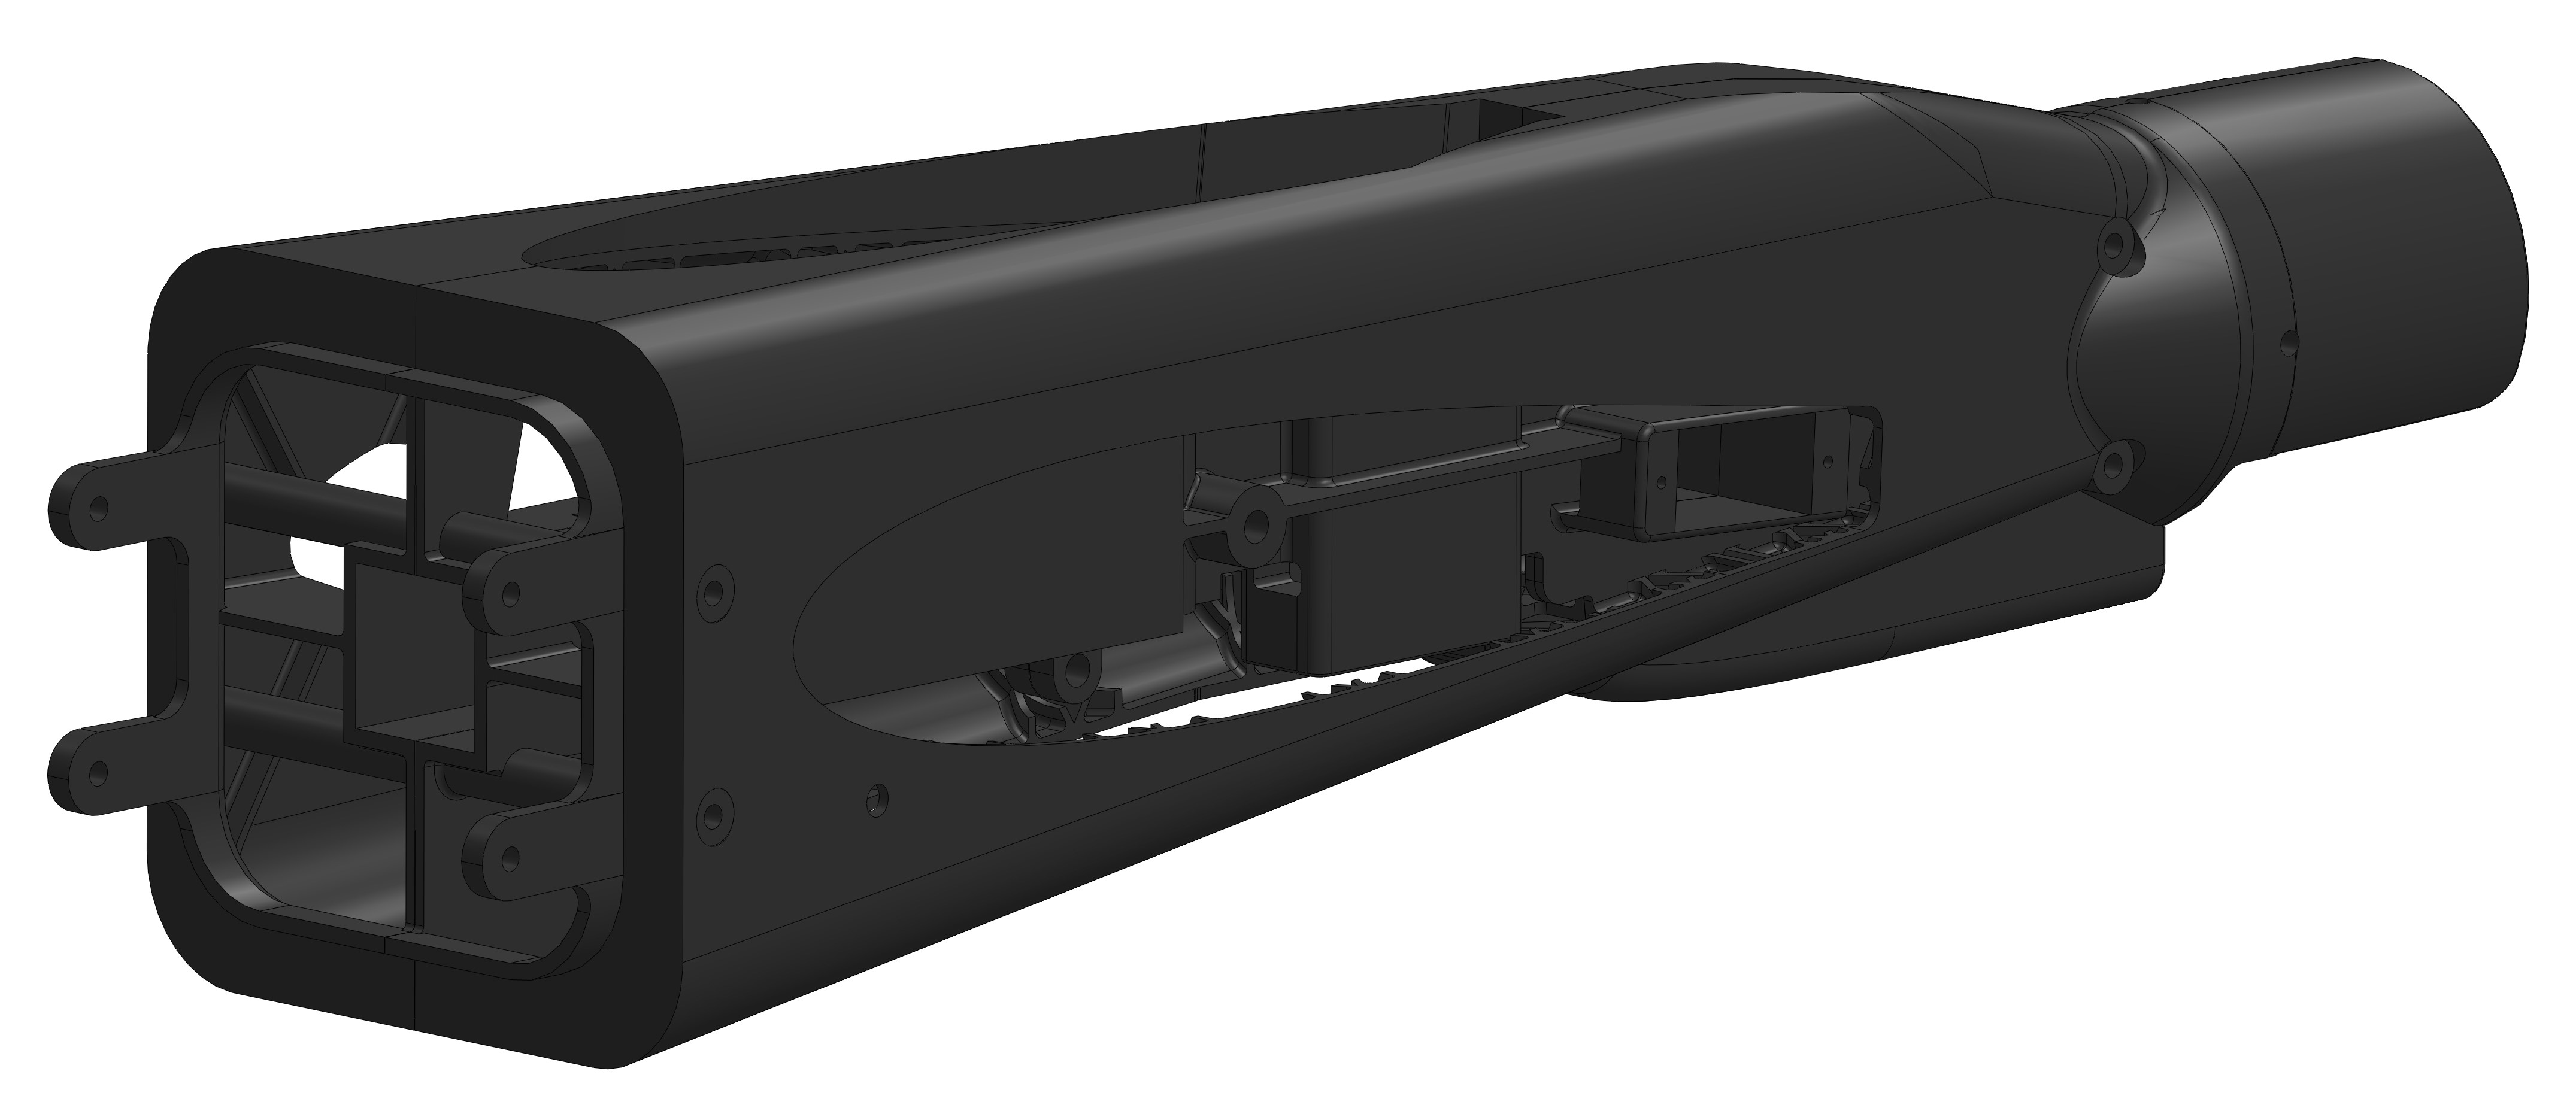
\includegraphics[width=\textwidth]{tail-mount-final}
        \caption{}
        \label{fig:tail-mount-design:whole}
    \end{subfigure}
    
    \caption{final tail mount design; (a) shows a cut view.}
    \label{fig:tail-mount-design}
\end{figure} 

\importimage{exploded-tail}{exploded view of the tail assembly, including fasteners.}{Exploded tail assembly}{0.7}

\section{Control surfaces} \label{sec:final-design-proposal:control-surfaces}

\subsection{Mathematical modelling} \label{sec:final-design-proposal:control-surfaces:mathematical-modelling}

The control surfaces were designed around their ability to meet several criteria that commercial aircraft must satisfy to be flyable. While this UAV isn’t required to meet the same stringent safety standards, many are there simply to ensure the aircraft flies properly, so it was prudent to meet them, a such, the rudder was designed to maintain trim control in the unlikely event of a wing tip motor failing resulting in worst case asymmetric thrust.  

To begin, the rudder was parameterised in terms of the ratio of it’s chord to the root chord of the vertical stabiliser, it’s span, and it’s inside offset from the root of the stabiliser allowing space for the servo.
Several useful parameters were derived from this including the MAC ratio, which was used on a plot from (Sadraey, 2013) to find the angle of attack effectiveness ($tau$) of the rudder, which was used to calculate the rudder control derivative using equation 12.100 in (Sadraey, 2013).
The rudder was modelled to be functioning at the predicted stall speed of the aircraft as it would be expected to maintain control at this speed.
A maximum deflection of 30 degrees was selected based (Sadraey, 2013), then this and relevant values substituted into equation 12.104a in (Sadraey, 2013) to calculate the vertical stabiliser lift with a deflected rudder. 

The first version of this with only the upper vertical stabiliser yielded a lift of 5.08 N.
This required comparing to the moment from the tip motor at full thrust, at stall speed.
The thrust of the motor changes with the inflow velocity.
Analysis of motor test data gave the thrust at predicted stall speed to be 8.73 N.
The wing has a semi-span of 1 m, so this is equal to the moment theoretically created in an asymmetric thrust scenario at this speed.
The tail arm was initially to be 1 m, but was reduced to 0.9 m for the purpose of moving the centre of mass forward, giving a tail moment of 4.57 Nm, which is approximately half of that required by the asymmetric thrust scenario.
This design flaw, combined with the fact that the rear propeller in that configuration would be unprotected on rotation or a hard landing, led to the decision to add a lower vertical stabiliser, despite it being surplus required vertical stabiliser area. 

The upper stabiliser was extended very slightly, the same root and tip chords maintained for upper and lower stabilisers, and simply a span extended below the fuselage until it extended approximately an inch beyond the lowest reach of the rear propeller, visible in figure 53. 

The values of both spans were altered until the force created by the deflected rudder was sufficient to counteract the moment from the asymmetric thrust.
The increase of the span had the effect of increasing the effective aspect ratio of the vertical stabiliser, which increased the efficiency, and thus the 3D lift curve slope, so it wasn’t required to simply double the area. 

The calculation was run with different speed values in Excel, to plot the rudder effectiveness and the motor thrust moment, over the expected speed range of the UAV: 

\importimage{rudder-thrust-moment}{rudder against thrust moment at various speeds.}{Rudder against thrust moment}{0.95}

With this requirement satisfied, design of the rudder was concluded.
The lack of runway landing and already excessive rudder size lead to the decision to forgo other rudder validation tests. 

The next stage of the design was the elevators, which began with parameterized geometry of the elevator through a root chord ratio.
A value of a quarter chord was selected initially, and this proved to be more than sufficient for all subsequent analyses, so remained.
The elevators took up all available trailing edge span of the horizontal stabiliser, leaving only room for the servo required to control it.  

The first attempt at the analysis of required deflections implemented a MATLAB code from (Sadraey, 2013) section 12.8.2, in Excel, to plot out the elevator deflections for the most fore and aft centre of gravity, and over the predicted speed range of the UAV.
The output of this code appeared to not be able to capture the 0 elevator deflection required at cruise speed (as the tail mounting angle has been designed around this).
Prof. Towell provided another method to try before assuming that the tail mounting angle calculations were wrong.  

The process given started with a moment balance about the centre of gravity of the aircraft including lift, tail lift, wing pitch moment equated to the tail lift moment.
This could have values substituted in for lift, and be rearranged for the tail lift coefficient: 

\importequation{
    C_{L_h} = \frac{q S C_L (h-h_0) c + T z_T + q S C_{M_0}}{q S_h l}
}{cog-moment-balance}

Then performing analysis of forces in vertical equilibrium, rearranging and substituting for the tail lift coefficient above  and rearranging for alpha, yielded the fuselage angle of attack at a given cruise condition: 

\importequation{
    \alpha = \frac{2 (mgl - Tz_T) V^{-2} - c C_{M_0}}{\rho S C_{L_\alpha}(l + (h - h_0)c)}
}{vertical-equilibrium}

With alpha found for a range of speeds, it could be used to find the tail lift coefficient for that particular speed, which is found by a rearranged version of the equation for tail lift coefficient, noting $\frac{S_h l}{Sc} = \overline{V}_h$, yielding: 

\importequation{
    C_{L_h} = \frac{C_{L_\alpha}\alpha(h-h_0) + \frac{Tz_T}{qSc} + C_{M_0}}{\overline{V}_h}
}{rearranged-tail-lift-coefficient}

With this, the elevator deflection can finally be calculated using:

\importequation{
    \delta = \frac{C_{L_h}}{C_{L_{\alpha_h}}} - \alpha (1 - \epsilon_\alpha) - \epsilon_0 - \frac{\alpha_h}{\tau_e}
}{elevator-deflection}

The process used above, along with the failed MATLAB code, repeated for a range of speeds yielded this plot (see legend for details):

\importimage{elevator-deflection}{elevator deflection plots for both processes.}{Elevator deflection plots}{0.95}

The second process captured the 0 deflection required at cruise speed, and appeared to be correct, so design was concluded as satisfactory in this case.
Additionally the deflections required from below the stall (and take off) speed are within the maximum deflections of the elevator selected.
The last test for the elevator was that it was satisfactory for aircraft rotation performance, which was based on a process from section 12.8.2 in (Sadraey, 2013), and involved determining all forces and moments on the aircraft for the elevator to overcome on aircraft rotation.
To begin, the take-off induced drag factor was determined using equation 5.22 in (Sadraey, 2013), then this and other pre-determined values were used to determine the take-off drag coefficient using equation 5.68 from (Sadraey, 2013).
This was then used to determine the take-off drag using the basic drag equation at a take-off speed of 13 m s-1 and a value of 11.56 N was calculated.  

Next the pitching moment about the aerodynamic centre was estimated as the wing 0 lift pitch moment coefficient, and then a basic pitch moment equation to determine the moment on take-off as -2.55 Nm.
The aircraft’s linear acceleration on rotation was then determined using equation 12.55 from (Sadraey, 2013) with an estimated friction coefficient of grass from Table 9.7 in (Sadraey, 2013). 

Next, several geometric parameters of the aircraft were determined from the CAD model to be then substituted into equation 12.72 in (Sadraey, 2013) to determine the lift required of the tail to achieve a set angular acceleration given the aircraft’s mass moment inertia about the pitch axis.
This yielded a tail lift of -3.17 N, which gave a tail lift coefficient of -0.192.
Checking using the method defined previously to determine the elevator deflections at various speeds gave+ a required deflection of -7.59o, which is less than the maximum of -25o, so this is acceptable.
This concluded elevator design. 

Finally, the ailerons required sizing.
This was based around their ability to reach a required roll angle within a set time.
This requirement varies based on the aircraft type and flight phase, which was determined from table 12.12b in (Sadraey, 2013) as a class II at phase C, at level 1.
The ailerons were parameterized by chord ratio (beginning with a value of 0.25, which proved satisfactory, so remained), and their inboard and outboard spans, however these were limited by the motor mount locations, so the main value to iterate upon was the chord ratio.  

A process from section 12.8.1 of (Sadraey, 2013) was used to determine aileron performance, beginning with the determination of the angle of attack effectiveness of the ailerons using the same method as previously.
This and several parameters were used in equation 12.23 from (Sadraey, 2013) to determine the aileron rolling moment coefficient derivative, yielding a value of 0.273 rad s-1, which was then used to determine the aileron rolling moment coefficient at the maximum deflection of the aileron using equation 12.13 in (Sadraey, 2013), which gave a value of 0.095. 

The ailerons need to be effective at an estimated approach velocity of 1.1 times the stall speed.
The aileron lift was then determined using equation 12.11 in (Sadraey, 2013) which resulted as 10.04 N.
This was then used to determine the steady state roll rate using equation 12.37 in (Sadraey, 2013), which gave a value of 7.14 rad s-1, which was then used to determine the bank angle at which the steady state roll rate would be achieved, using equation 12.43 in (Sadraey, 2013), which gave a value of 74.57 degrees.
The rate of roll rate could then be calculated using equation 12.49 in (Sadraey, 2013), which gave a value of 0.342 rad s-2.
Finally, the time to reach a bank angle of 30 degrees could be calculated using equation 12.47 in (Sadraey, 2013), which resulted as 1.75 seconds, less than the maximum 1.8 seconds, so the aircraft satisfied roll control requirements.
The time reduced to 1.17 seconds for the same process repeated at cruise speed. 

To conclude control surface mathematical design, it was checked using XFOIL that the servos chosen would be able to cope with the hinge moments.
For aesthetics it was chosen to have the servo axis in line with the control surface axis.
This removes the need for horn controls.
A code was used that yielded a hinge moment coefficient, which was then multiplied by relevant values to obtain the hinge moment.
As the servo and control surface axes were in line, if this value was greater than the stall torque of the servo, the servo was deemed inappropriate.
The SG90S had been selected, and was appropriate for all control surfaces, apart from the upper rudder, which was later changed to a HITEC HS 85 MG servo, which had sufficient stall torque. 

\subsection{CAD modelling} \label{sec:final-design-proposal:control-surfaces:cad-modelling}

% \importimage{elevator}{a single elevator.}{Elevator}{0.4}
% \importimage{transparent-stabiliser}{a transparent view of the assembly of one horizontal stabiliser and elevator.}{Horizontal stabiliser}{0.4}

\begin{figure}[H]

    \centering
    \begin{subfigure}[b]{0.49\columnwidth}
        \centering
        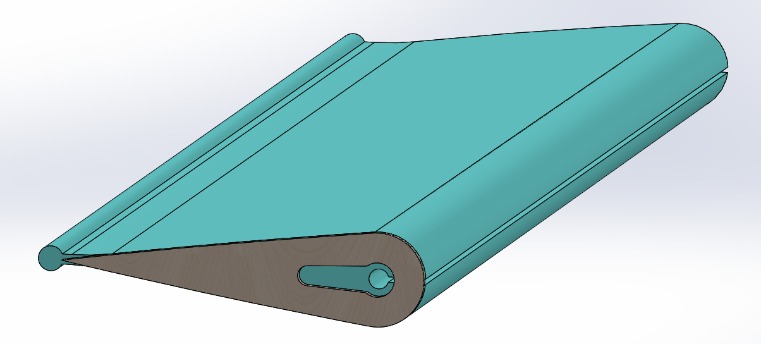
\includegraphics[width=\textwidth]{elevator}
        \caption{Elevator}
        \label{fig:tail-assembly:elevator}
    \end{subfigure}
    \hfill
    \begin{subfigure}[b]{0.49\columnwidth}
        \centering
        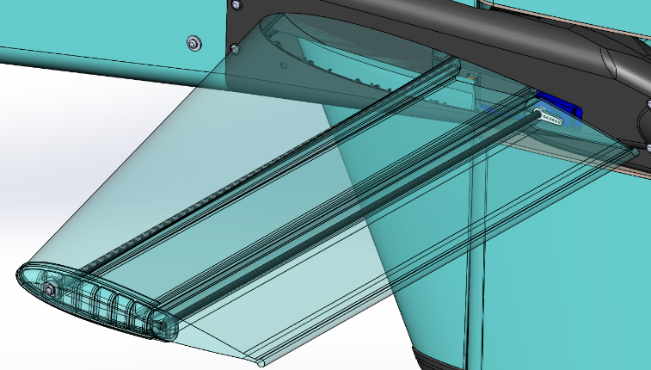
\includegraphics[width=\textwidth]{transparent-stabiliser}
        \caption{Horizontal stabiliser}
        \label{fig:tail-assembly:horizontal-stabiliser}
    \end{subfigure}
    
    \caption{components of the horizontal component of the tail section.}
    \label{fig:tail-assembly}
\end{figure} 

The rudder basic shape was cut out from a duplicate of the vertical stabiliser model.
The space for the servo was cut out from the root, then additional cut-outs made for the stiffening spar near the leading edge, and foam cutter wire paths.
Next a thin second body was extruded from the root to define a laser cut profile that would allow for the servo arm to have a place to nest into, allowing for control of the rudder.
Lastly a small circular profile (designed to be cut off manually later) was extruded on the trailing edge so that the foam cutter would not damage the trailing edge since it was so thin.
The secondary rudder and elevators were defined identically. 

The ailerons were generated from a sketch of the aerofoil profile which was defined from the wing profile sketch, then one aileron extruded in a long profile, then, planes were defined in the model that referenced the motor mount surfaces in contact with the aileron root and tip surfaces.
Material outside of these two planes was then removed to define one aileron, which was then mirrored about the centre plane, defining both ailerons in a way that would instantly react to changes in motor mount location and spans between them.
Next a small amount was cut off the roots of the ailerons and replaced with a small laser cut profile extruded outwards, similarly to the tail control surfaces that allowed for the inline servo arm to control the aileron.
Finally, holes were added for a stiffening spar, and wire paths added for the foam cutter. 

\section{Electronics} \label{sec:final-design-proposal:electronics}

% TODO: split into subsubsections

The avionics of the aircraft were meant to fulfil two main goals.

\begin{itemize}
    \item Provide the pilot with assistance in flying the aircraft using a flight controller, generally maintaining stability. 
    \item Have basic autopilot functionality, allowing the aircraft to fly in straight and level flight at a consistent speed to enable the fair testing of different flight configurations. 
\end{itemize}

As well as this, the avionics would be required to extend and retract the flaps, and ideally to record data - specifically on the rate of battery drainage. 

The primary role of the flight controller is to convert control inputs from the pilot into control inputs that are sent directly to the servos, and is normally accomplished through a range of techniques, including PID controllers.
Two main flight controllers were investigated, the first being a Pixhawk flight controller - more expensive, but potentially more useful and had been used by people at the university before - and the second being a Matek F405-Wing board with iNav Flight firmware installed on it. 

While the Pixhawk could have been easier to set up, with its advertised “plug and play” functionality, it was significantly more expensive, and it was decided that looking into the Matek controller could be worth a potentially large saving, albeit with a greater risk of purchasing the controller to find that it did not work as expected.
The Matek hardware came at about half the cost, and while the corresponding firmware was relatively immature, its open source nature meant that its functionality was expanding quickly, and it had favourable reviews from a number of online sources.
Another potential advantage of the Matek controller was that it was designed specifically with fixed wing aircraft in mind, whereas the Pixhawk was focused more towards quadcopters. 

\importimage{matek}{pin layout and documentation for the Matek flight controller.}{Flight controller layout}{0.95}  % TODO: include source (http://www.mateksys.com/?portfolio=f405-wing)

Other beneficial features of the Matek board were the built-in current sensor and inertial measurement unit (IMU) which would provide estimates of the position, and more importantly orientation, of the UAV.
There were also a number of fairly low-cost GPS and airspeed sensor units, required for the latter part of the avionics system’s brief of providing autopilot functionality. 

\importimage{flight-configurator}{flight configurator software used to set up the flight controller.}{Flight configurator}{0.6}

Input to the flight controller could be achieved through a number of systems, most notably through SBUS; this type of serial connection appeared to be the most commonly supported amongst receivers, and would allow up to sixteen channels to be passed from the receiver to the controller.
The minimum required channels would be eight: four for throttle, yaw, pitch, and roll; two for flaps (on/off); and similarly two for the autopilot toggle.
With the additional channels it would in principle be feasible to implement extra features, such as manually cutting off outboard motors in the event that one of them should fail. 

Also of interest were the UART ports, which is a serial communication protocol broadly compatible with a number of microcontrollers, including Arduinos.
This would be a good option for extracting the data from the current sensor and passing it to a microcontroller - most likely an Arduino Nano - which could then integrate the current draw over time to provide an estimate of the battery capacity used by a particular configuration.
Being able to do this onboard was appealing because the need for telemetry, which would have significantly increased the complexity of the radio system, could be removed.
All data could be logged by a relatively simple program, written in C++, which could then be downloaded after each flight. 

\importimage{flight-controller-computer}{flight controller plugged into a computer running the flight configurator.}{Flight controller configuration}{0.6}
\importimage{flight-controller-receiver}{receiver undergoing the binding procedure.}{Receiver binding}{0.5}

While a Futaba transmitter was originally to be loaned from the university, scheduling constraints resulted in its unavailability for the duration of the project.
As an alternative, a FrSky Taranis X9D was purchased upon recommendation of its being a good tradeoff between price and flexibility.
The model is widely used and compatible with a wide range of receivers, uses a standard communication protocol, and also runs a configurable operating system, OpenTx, which enables it to be programmed in Lua.
As well as the standard joysticks, the handset has triggers and switches which can be mapped to the flaps and autopilot channels. 

Two primary factors constrained the selection of receiver.
The first was the output method, which needed to be SBUS to be compatible with the Matek flight controller, and have at least eight output channels.
The second was compatibility with the Taranis transmitter, which ruled out a number of Futaba receivers operating on a proprietary communication protocol. 

Other factors, while less important, included the power usage, cost, and size of the receiver.
The receiver was intended to fit onto an electronics tray along with the flight controller, and would be powered by the same battery as the flight controller, microcontroller, and servos.
A receiver, the FrSky X8R, was found, operating on 100mA at 5V (the standardised output voltage of the flight controller), and weighing less than 20g.
Its profile is also similar to that of the flight controller, meaning that it would not be the limiting factor in the size and shape of the electronics tray when the fuselage was designed. 

When bound to a Taranis X9D, the X8R is capable of receiving sixteen independent channels via FrSky’s radio transfer protocol ACCESS (a newer and more robust version of ACCST).
This would be more than sufficient for the eight channels required as a baseline for the project, and would also leave room for the expansion of the project with additional features, as mentioned previously, with the eight leftover channels.
The operating range of 1.5km would also be more than sufficient for the project. 

As well as being compatible with the Taranis transmitter and capable of outputting to SBUS, the receiver had a number of serial ports (standard PWM outputs) which could be used for testing and validating its functionality without having to pass the signals through the flight controller first.
It was thought that this could be useful in the later stages of the project while troubleshooting any issues, being able to remove the flight controller from the loop and isolate the receiver to check that it was communicating properly with the transmitter. 

All moveable surfaces on the aircraft are actuated by servos.
These are split into four groups: ailerons, elevators, rudder, and flaps.
The first three are the control surfaces by which the aircraft is controlled, and would need to be sized for a fairly limited selection of manoeuvres.
It was not expected that the aircraft would be performing any tight turns, but the load that would be transferred through the aileron servos could depend greatly on the configuration of the propulsion modules.
With the modules located at the end of the wings, the greatly increased moment of inertia of the aircraft would mean that actuating the ailerons would not produce nearly as much inertial relief as when the motors and batteries were located on the centreline.
As such, the servos could be expected to see a fairly variable range of loads.
In addition, the loads experienced by the rudder servos was found to be far in excess of the loads experienced by all other servos when the possibility of an asymmetric motor failure at the wingtips was considered.
It was decided that these servos would need to be of a different type to those elsewhere in the aircraft. 

In all, fourteen servos would be required to control the aircraft, including the two servos of different specification for the rudder.
The exact configuration of these servos, as well as the signals passed to each of them, is shown below. 

\importimage{signal-splitters}{control signal splitter schematic.}{Signal splitter schematic}{0.7}

Note that each flap is supported by two servos of opposing deflection directions.
While the flaps increase the lift of the aircraft quite dramatically, and thereby exert a large moment onto their supporting servos, the distribution of this load across four flap segments and eight servos meant that the smaller servo size was capable of holding the flaps in place during takeoff and landing. 

One potential issue with the servos selected was the degradation of the plastic-toothed gears they use.
Information from peers suggested that sufficient use would wear the gears down and reduce their effective strength, causing the gears to slide at a smaller load than suggested by the servos’ data sheets.
An experiment was devised to repetitively test a servo under load (actuating it far more times than would ever be expected of a servo in a flight model) to see whether its strength afterwards was the same as upon its delivery; but this experiment was never carried out due to the COVID-19 pandemic.
In the event that it had been found to significantly impact the strength of the servos, metal-toothed servos could have been purchased at a slightly higher cost. 

The entirety of the electronics subsystem was to be powered by a single battery, referred to as the avionics battery.
This would be connected to the flight controller, powering it directly, and indirectly powering the receiver, microcontroller, and servos.
While throttle signals would be supplied to the motors from the flight controller directly, the bulk of their power would come from the ESCs, which are in turn powered by the battery local to that propulsion module. 

In order to size the battery used for the avionics, the approximate power draw of each of the electrical components needed to be determined.
Research was conducted, considering the following items drawing power during a typical 10-minute flight: 

\begin{itemize}
    \item Servos
        \begin{itemize}
            \item Draw 10mA while idle, 100-250mA while moving, and have a stall current of 360mA 
            \item The stall torque of the servos being used is 1.7kg.cm, meaning that for a 4cm control surface, a load of roughly 0.5kg would need to be applied to cause a stall.
                Considering that there are nine control surfaces and that the total lift generated by the aircraft is around 7kg, it can reasonably be assumed that the likelihood of any individual control surface experiencing a load of 0.5kg is extremely small; certainly small enough that it will occur only momentarily and does not need to be factored into the draw calculations 
            \item 8 servos are being used for the flaps and so will only move for a few seconds per flight 
            \item One servo connected to the nose gear, which will likely only be moving periodically within two 30-second windows at the start and end of each flight 
            \item 5 servos are connected to the control surfaces.
                It is assumed that control surfaces will only move for around 50\% of the time while in the air.
                To build in a bit of redundancy and account for the movement of the flap/gear servos, it is assumed that the power drain from servos will be equivalent to five servos moving constantly 
            \item This then means 1000mA drawn by servos 
        \end{itemize}
    \item Receiver: listed as drawing a continuous 100mA 
    \item Flight controller: listed as drawing a continuous 500mA, a conservative estimate 
    \item The exact current draw of a microcontroller is difficult to determine as it depends primarily on how much the processor is being used.
        Even conservative estimates resulted in around 20mA of draw, so that was neglected here as it is so much smaller than the other components 
\end{itemize}

An additional constraint placed on the battery was the required voltage of between 9 and 30 volts.  As the battery needs to be a LiPo battery, this limited the selection to those with between 3 and 6 cells. 

Given a total of 1600mA drawn while in flight (a conservative estimate which also accounts for the small amount of additional power used for one-off events during takeoff and landing), and the voltage requirements, a few batteries were found which could power the avionics.
Several higher-capacity batteries were heavier and more expensive and, while they would enable multiple flights on one battery, switching out multiple lower-capacity batteries which were both lighter and cheaper was found to be more cost- and mass-effective, and also in keeping with the modular nature of the project. 

The battery settled on was therefore a 450mA, 11.1V, and 65-130C discharge, which should provide for at least 15 minutes of flight on a conservative estimate of the power draw.
Its low cost means that multiple can be bought and swapped out between flights, while used batteries are recharged. 

With all the components of the avionics subsystem specified, a wiring diagram could be created and from this an iron bird constructed.
The primary goal of this exercise was to check that every required component was present, and that they would all fit together with the necessary wires. 

\importimage{wiring-diagram}{wiring diagram for the avionics subsystem.}{Wiring diagram}{0.6}

From the above diagram, the iron bird was built onto a miniaturised cutout of the same general shape as the full-size aircraft. 

\importimage{iron-bird}{iron bird.}{Iron bird}{0.7}

While not all of the servos were included in the iron bird, each servo group was represented.
The iron bird also gave a much clearer indication of roughly how much wiring would be needed to connect the various groups, and which layout would be most efficient for splitting the signals; that is, which signals should be brought down each of the main “limbs” of the aircraft, and where should they be split.
Once this was decided, the splitters could be designed and manufactured. 

\importimage{splitter-schematic}{manufacturing schematic for a single splitter.}{Manufacturing schematic}{0.5}

A schematic similar to the one shown above was drawn out for each of the splitters identified in Figure \ref{fig:splitter-schematic}.
This includes the specification of the splitter in terms of the signals designated as inputs and outputs, and shows its layout in terms of header pins (rectangular boxes) soldered (ovals) across a stripboard whose strips are assumed to go across the page horizontally.
Breaks in the stripboard are shown here by small vertical lines instead of a dot representing the corresponding hole. 

These splitters were manufactured from small cut segments of stripboard by simply soldering header pins in the correct locations.
The seven splitters also had small outcrops of stripboard so that they could be fastened to relevant locations throughout the body of the aircraft. 

\importimage{manufactured-splitters}{each of the manufactured splitters.}{Manufactured splitters}{0.8}

Although the full electronics system was never assembled in the UAV due to the COVID-19 pandemic, all of the necessary physical components were purchased and manufactured, and their compatibility was tested in the iron bird. 

% \importimage{electronics-housing}{render of the electronics housing bay in the tractor nose propulsion configuration.}{Electronics housing}{0.4}
% \importimage{electronics-exploded}{exploded view of the avionics subsystem.}{Avionics subsystem}{0.4}

\begin{figure}[H]
    \centering
    \begin{subfigure}[b]{0.49\columnwidth}
        \centering
        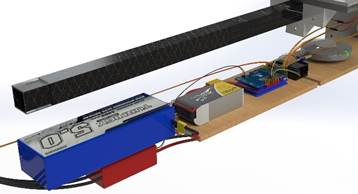
\includegraphics[width=\textwidth]{electronics-housing}
        \caption{Housing bay}
        \label{fig:electronics-subsystem:bay}
    \end{subfigure}
    \hfill
    \begin{subfigure}[b]{0.49\columnwidth}
        \centering
        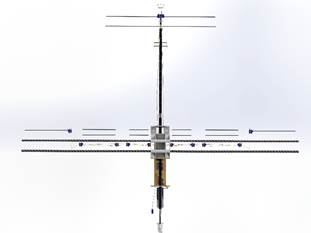
\includegraphics[width=\textwidth]{electronics-exploded}
        \caption{Subsystem, exploded}
        \label{fig:electronics-subsystem:exploded}
    \end{subfigure}
    
    \caption{renders of the key parts of the electronics subsystem.}
    \label{fig:electronics-subsystem}
\end{figure} 

\importimage{bixler}{image of the Bixler 3 RC plane.}{Bixler model}{0.5}

Before the electronics were to be flown on the UAV, they needed to be tested.
There was thorough testing of the electronics out of any aircraft first, but in order to be deemed flight worthy it needed to be tested in the air in a sacrificial flight vehicle.
The foamy selection was based on the constraints of the fuselage size required in order to have room to fit all of the electronics inside, keeping the cost as low as possible, and having an aircraft that we could fly ourselves (easy to fly for beginners).
The fuselage needed to be able to fit all of the necessity electronics; battery, ESC, receiver, as well as our additional electronics to control the autopilot; Arduino, Matek, and GPS.
Therefore we needed a beginners plane that had excess fuselage space, and so we chose the Bixler 3 as it has a large internal space for the necessity electronics, as well as an empty nose for installation of a camera for FPV flying, and this space would be suitable for fitting in our additional electronics.
Additionally the plane is designed for beginners and so has a large surface area wing for low speed flying, high mounted for flight stability, the motor and propeller face rearwards above the fuselage to get them out of the way of damage in the event of a crash, and the underside of the fuselage is strengthened to act as a skid if the landing gear comes off in a particularly heavy landing.
All of this makes it ideal for our use case.
However, it was not flow due to the coronavirus lockdown, and so the electronics could not be flight tested. 

\section{Avionics and software} \label{sec:final-design-proposal:avionics-and-software}

% TODO: populate from electronics section

\section{Propulsion} \label{sec:final-design-proposal:propulsion}

The design of the housing for the motors and its subsidiary systems focused on permitting the repositioning of these system in a small time window without the need for alteration to the design.
Thus increasing the amount of flights which can be completed in one day.
This was crucial so that the difference in atmospheric conditions are reduced to minimum. 
A self-contained housing storing the motor, the ESC and the battery was designed; referred as ‘Power Unit Cell’ (PUC).
The use of such design allowed the reduction of wires running through the wing as well as making those components more accessible for maintenance.
Furthermore, the use of a compact design allowed for a standard PUC which could be used in all wing propulsion configurations.
This was achieved by creating a standard simple profile for the surfaces normal to the attachment points; this is evident in Fig. 12.
In order to guarantee a smooth passage of the flow around the housing an adapter is created for each configuration.
This slots onto the standardized surfaces of the power unit cell and mounts directly on the wing surfaces blending the two together.
Furthermore, they ensure that the thrust line in unvaried between tractor and pusher configurations. 

% \importimage{puc-tractor}{PUC section view in top-tractor configuration.}{PUC top tractor}{0.5}
% \importimage{puc-pusher}{PUC section view in top-pusher configuration; yellow is the adaptor, green is the ESC, red is the battery, and blue is the motor.}{PUC top pusher}{0.5}

\begin{figure}[H]
    \centering
    \begin{subfigure}[b]{0.49\columnwidth}
        \centering
        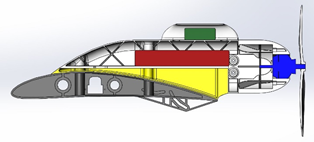
\includegraphics[width=\textwidth]{puc-pusher}
        \caption{Overwing pusher}
        \label{fig:puc-assemblies:pusher}
    \end{subfigure}
    \hfill
    \begin{subfigure}[b]{0.49\columnwidth}
        \centering
        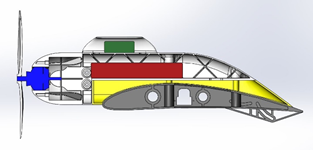
\includegraphics[width=\textwidth]{puc-tractor}
        \caption{Overwing tractor}
        \label{fig:puc-assemblies:tractor}
    \end{subfigure}

    \begin{subfigure}[b]{0.7\columnwidth}
        \centering
        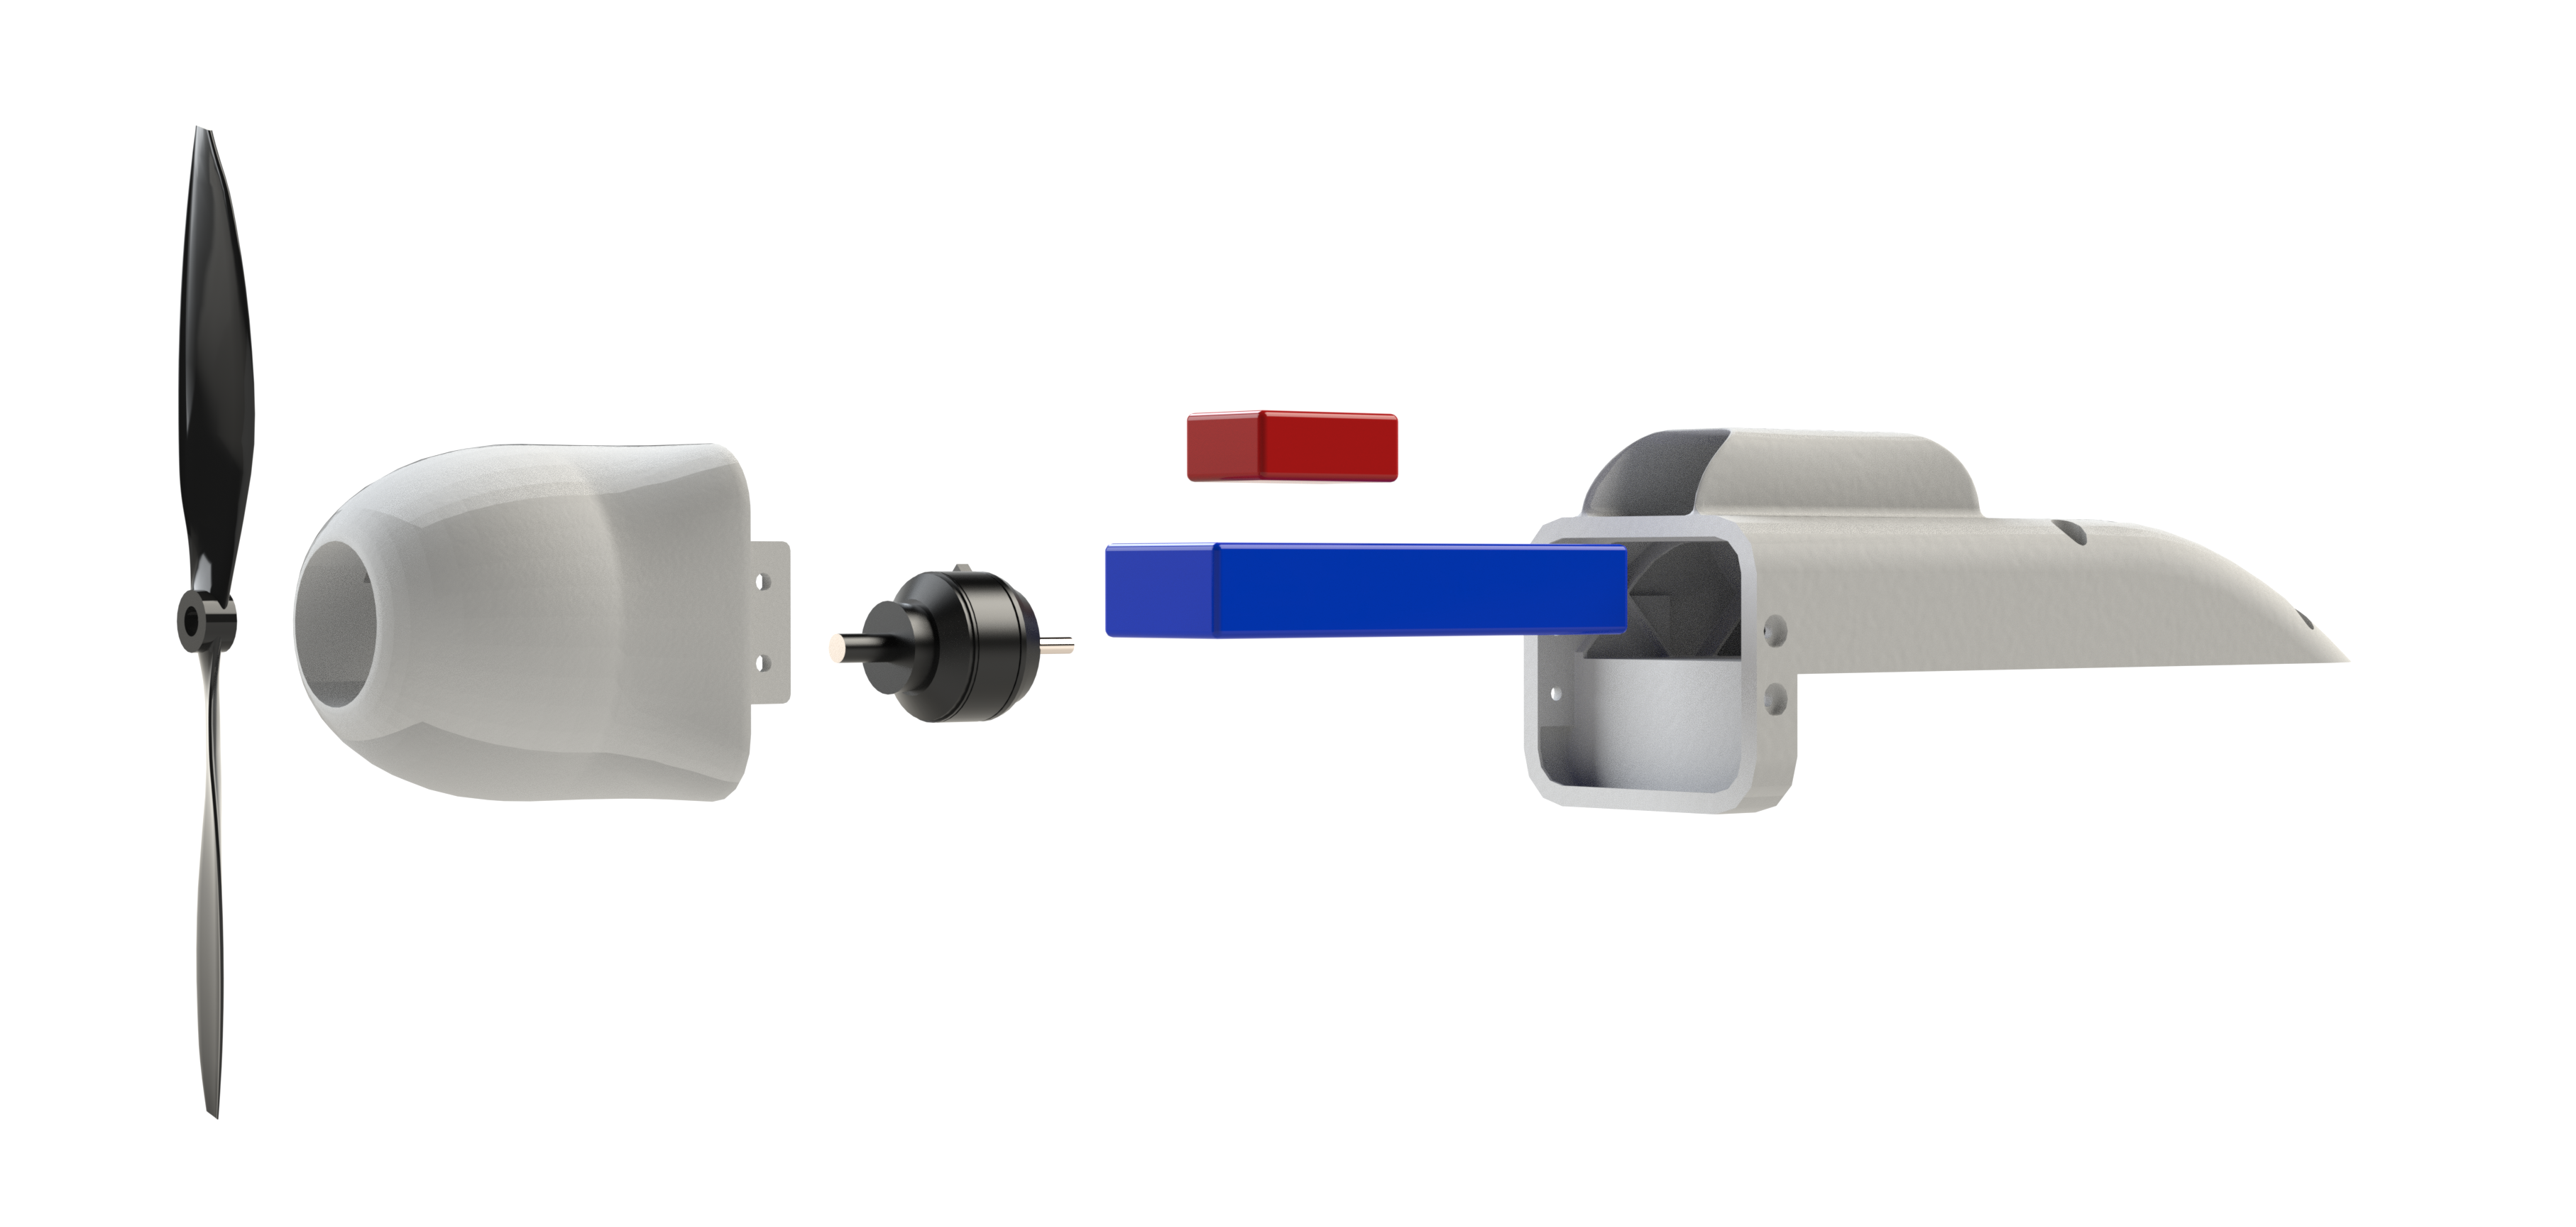
\includegraphics[width=\textwidth]{puc-exploded}
        \caption{Exploded}
        \label{fig:puc-assemblies:exploded}
    \end{subfigure}
    
    \caption{
        various views of the PUC assembly.
        Adapters are in yellow; ESCs are in green; batteries are in red; and motors are in blue.
    }
    \label{fig:puc-assemblies}
\end{figure} 

The distance from the trailing edge to the propeller in the pusher layout is equivalent to the distance from the leading edge to the propeller in the tractor layout.
Moreover, as in can be seen in Fig. 12.
The attachment holes for the mounting bolts remain in the same position despite the change in arrangement.
Hence, allowing to interchange propulsion layouts without the need of modifications to the components. 
The power unit cells are as well split in two components: a front section and a rear section.
Thus permitting to access the components stored inside with the removal of the four M4 bolts securing the two halves together.
Four threaded inserts imbedded in the nylon structure of the front section allow the fitting of the motor.
The battery and the ESC are instead slotted into the rear section of the cell.
The open section into which the ESC is placed ensures the cooling of this component in all configurations setup.
So to avoid common reliability issues caused by the overheating of this last.
An exploded view of the PUC assembly is shown in Fig. 13. 

% \importimage{puc-exploded}{exploded view of the PUC assembly.}{Exploded PUC}{0.6}

Due to the fitting of the battery and the ESC, the PUC assembly has a sensible weight.
In fact, as it will be discussed, the CG of the UAV is subject to a significant shift as the motor configuration is changed from tractor to pusher.
A reduction in this effect leads to a less significant need to rely on a ballast to maintain the CG in the same location. 
In order to reduce this effect, the battery was located in a closer position to half chord length with some compromises made for the aerodynamic aspect.
Furthermore, a work of light weighting of the components was carried.
Hence the use of ribs and reinforcements where loads concentrate and the use of thin walls shown in Fig. 14.
This resulted into an overall housing dry weight of 207g. 

% \importimage{puc-front}{PUC front section inner structure.}{PUC front section}{0.3}
% \importimage{puc-rear}{PUC rear section inner structure.}{PUC rear section}{0.3}

\begin{figure}[H]
    \centering
    \begin{subfigure}[b]{0.4\columnwidth}
        \centering
        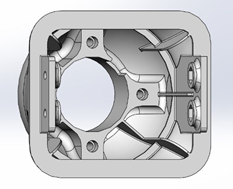
\includegraphics[width=\textwidth]{puc-front}
        \caption{Front}
        \label{fig:puc-design:front}
    \end{subfigure}
    \hfill
    \begin{subfigure}[b]{0.4\columnwidth}
        \centering
        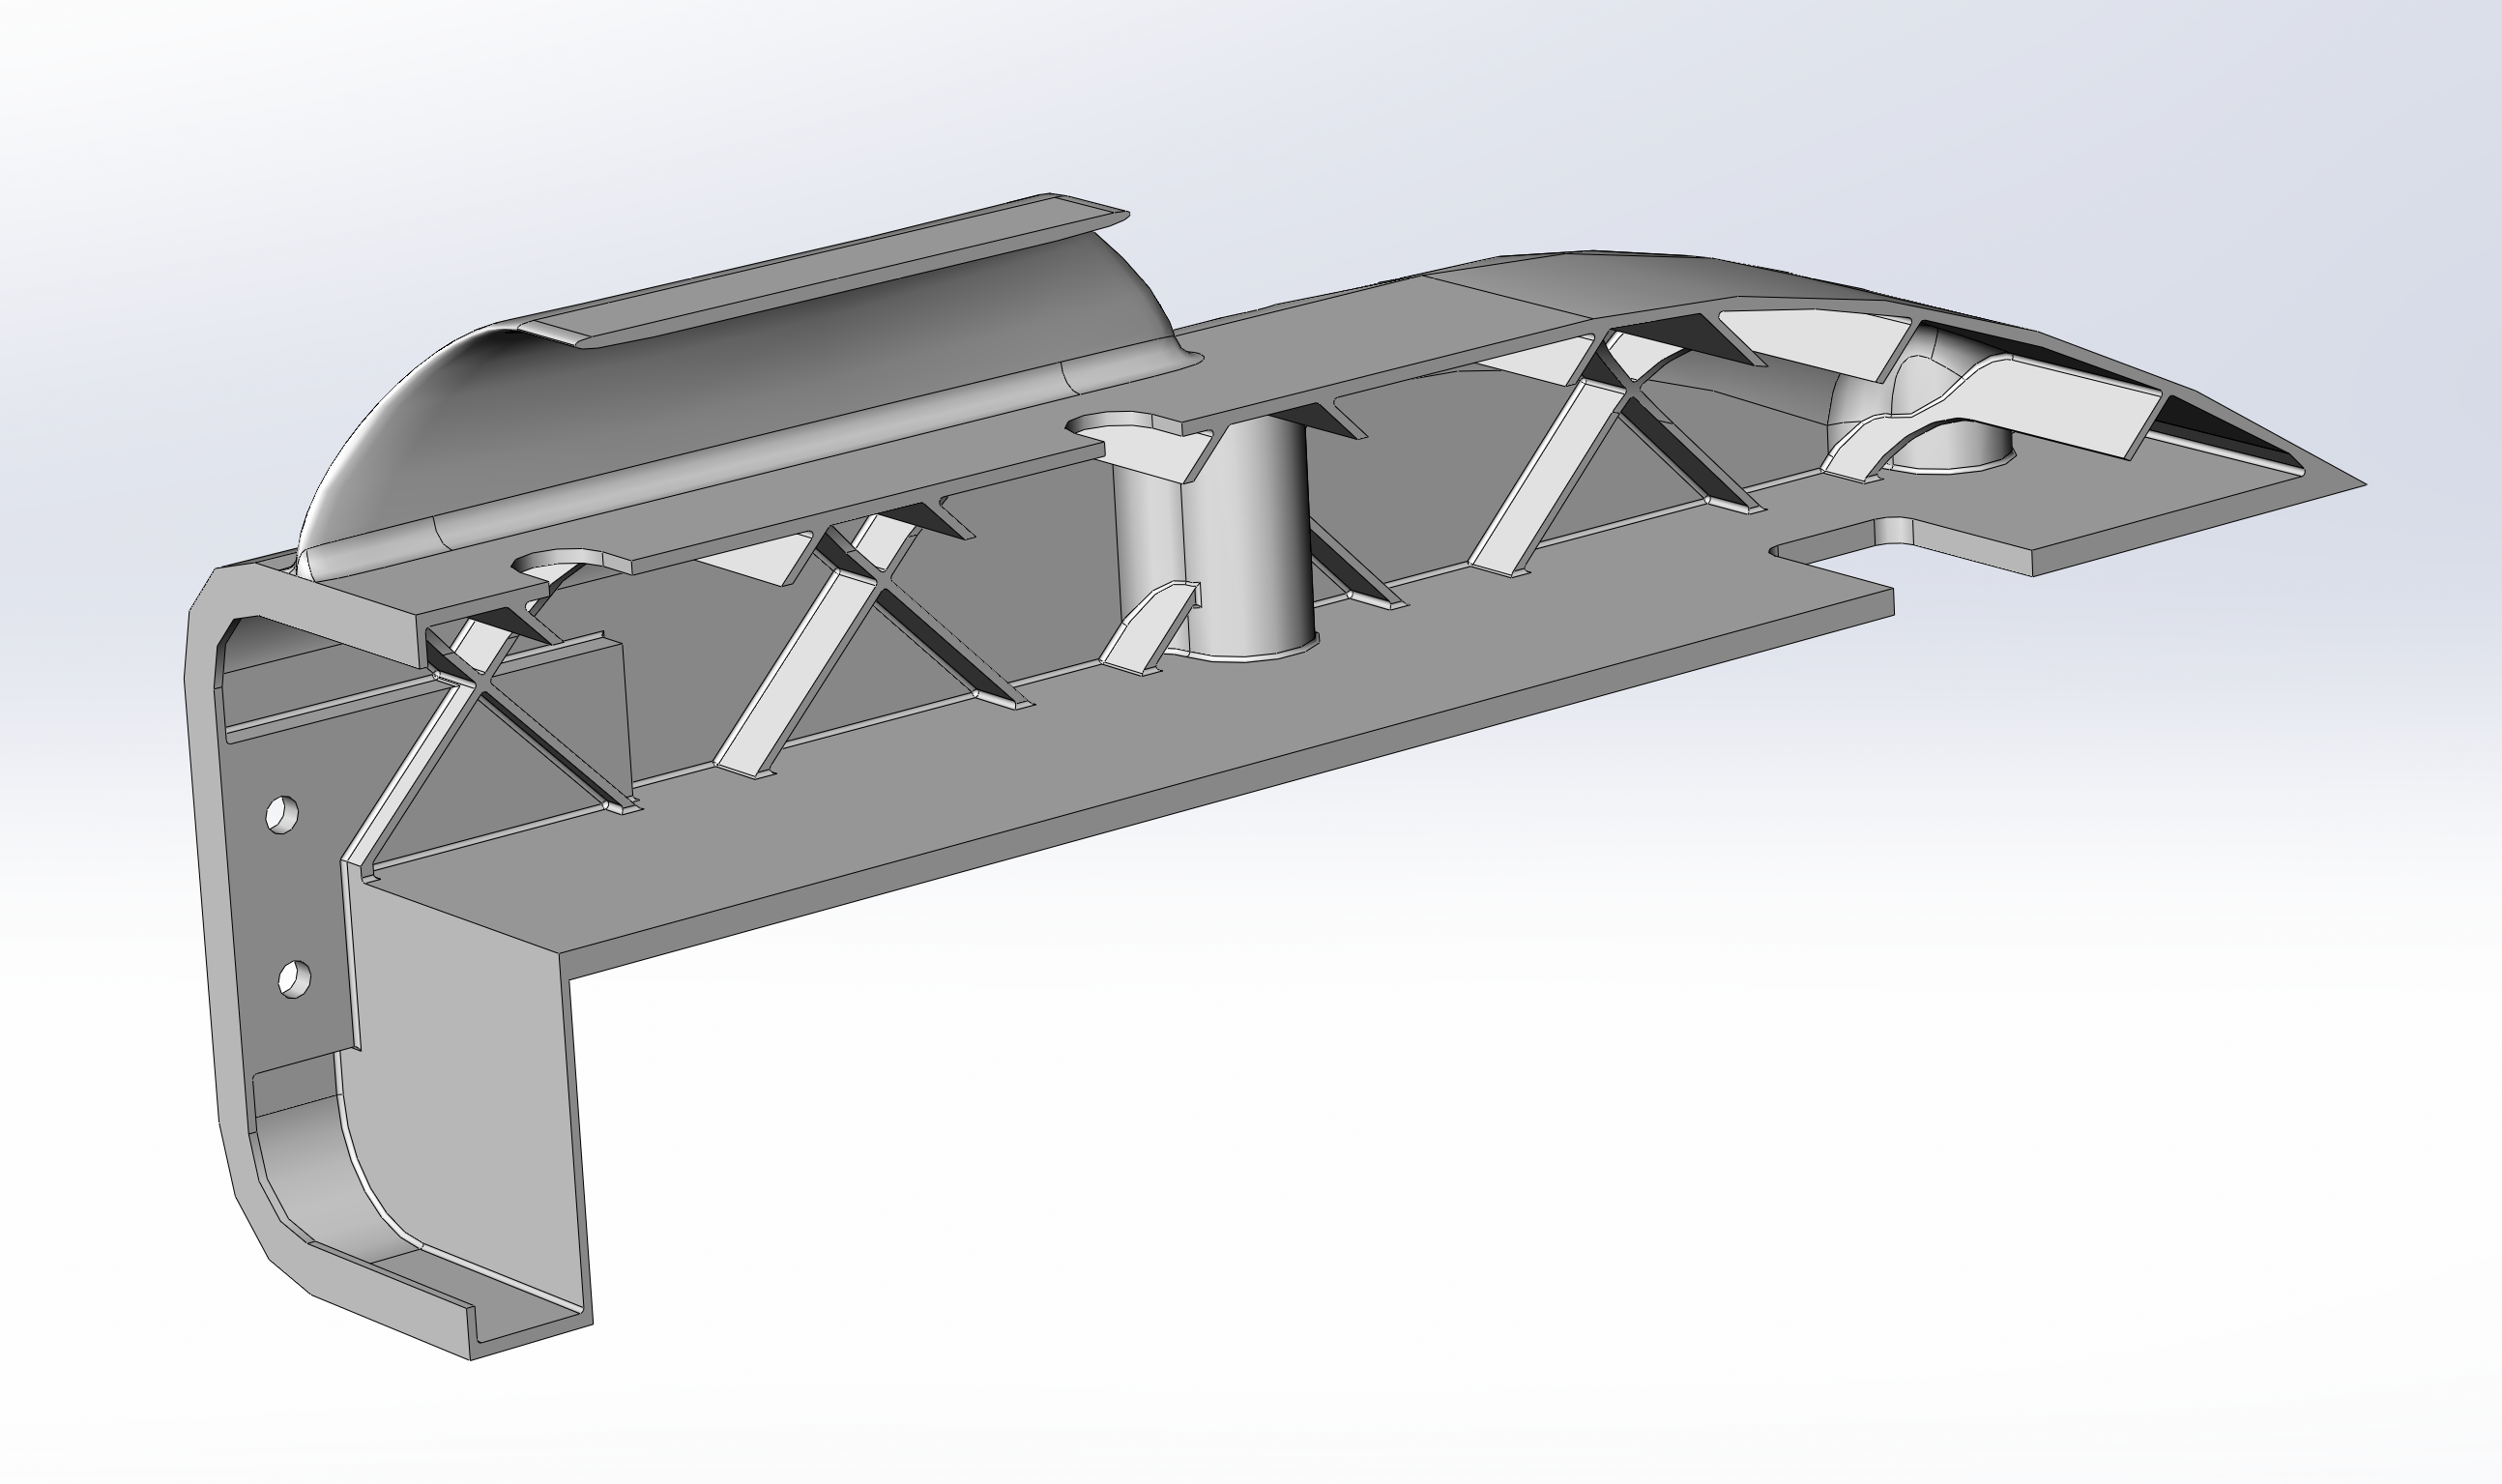
\includegraphics[width=\textwidth]{puc-rear}
        \caption{Rear}
        \label{fig:puc-design:rear}
    \end{subfigure}
    
    \caption{inner structure of the PUC.}
    \label{fig:puc-design}
\end{figure} 

\importimage{puc-printed}{PUC, printed in SLS nylon.}{SLS nylon PUC}{0.5}

\end{document}
